
\chapter{云边协同AI推理调度方法}

本章系统阐述了面向边缘计算与云计算协同场景的AI推理调度方法,该方法由两部分构成:云边协同AI推理调度模型、分层调度策略及算法。首先,本章概述了该方法的整体架构,并在此基础上详细概述了调度模型、分层调度策略和对各层的优化算法进行详细介绍。

\section{方法概述}







\begin{figure}[h]
  \centering
  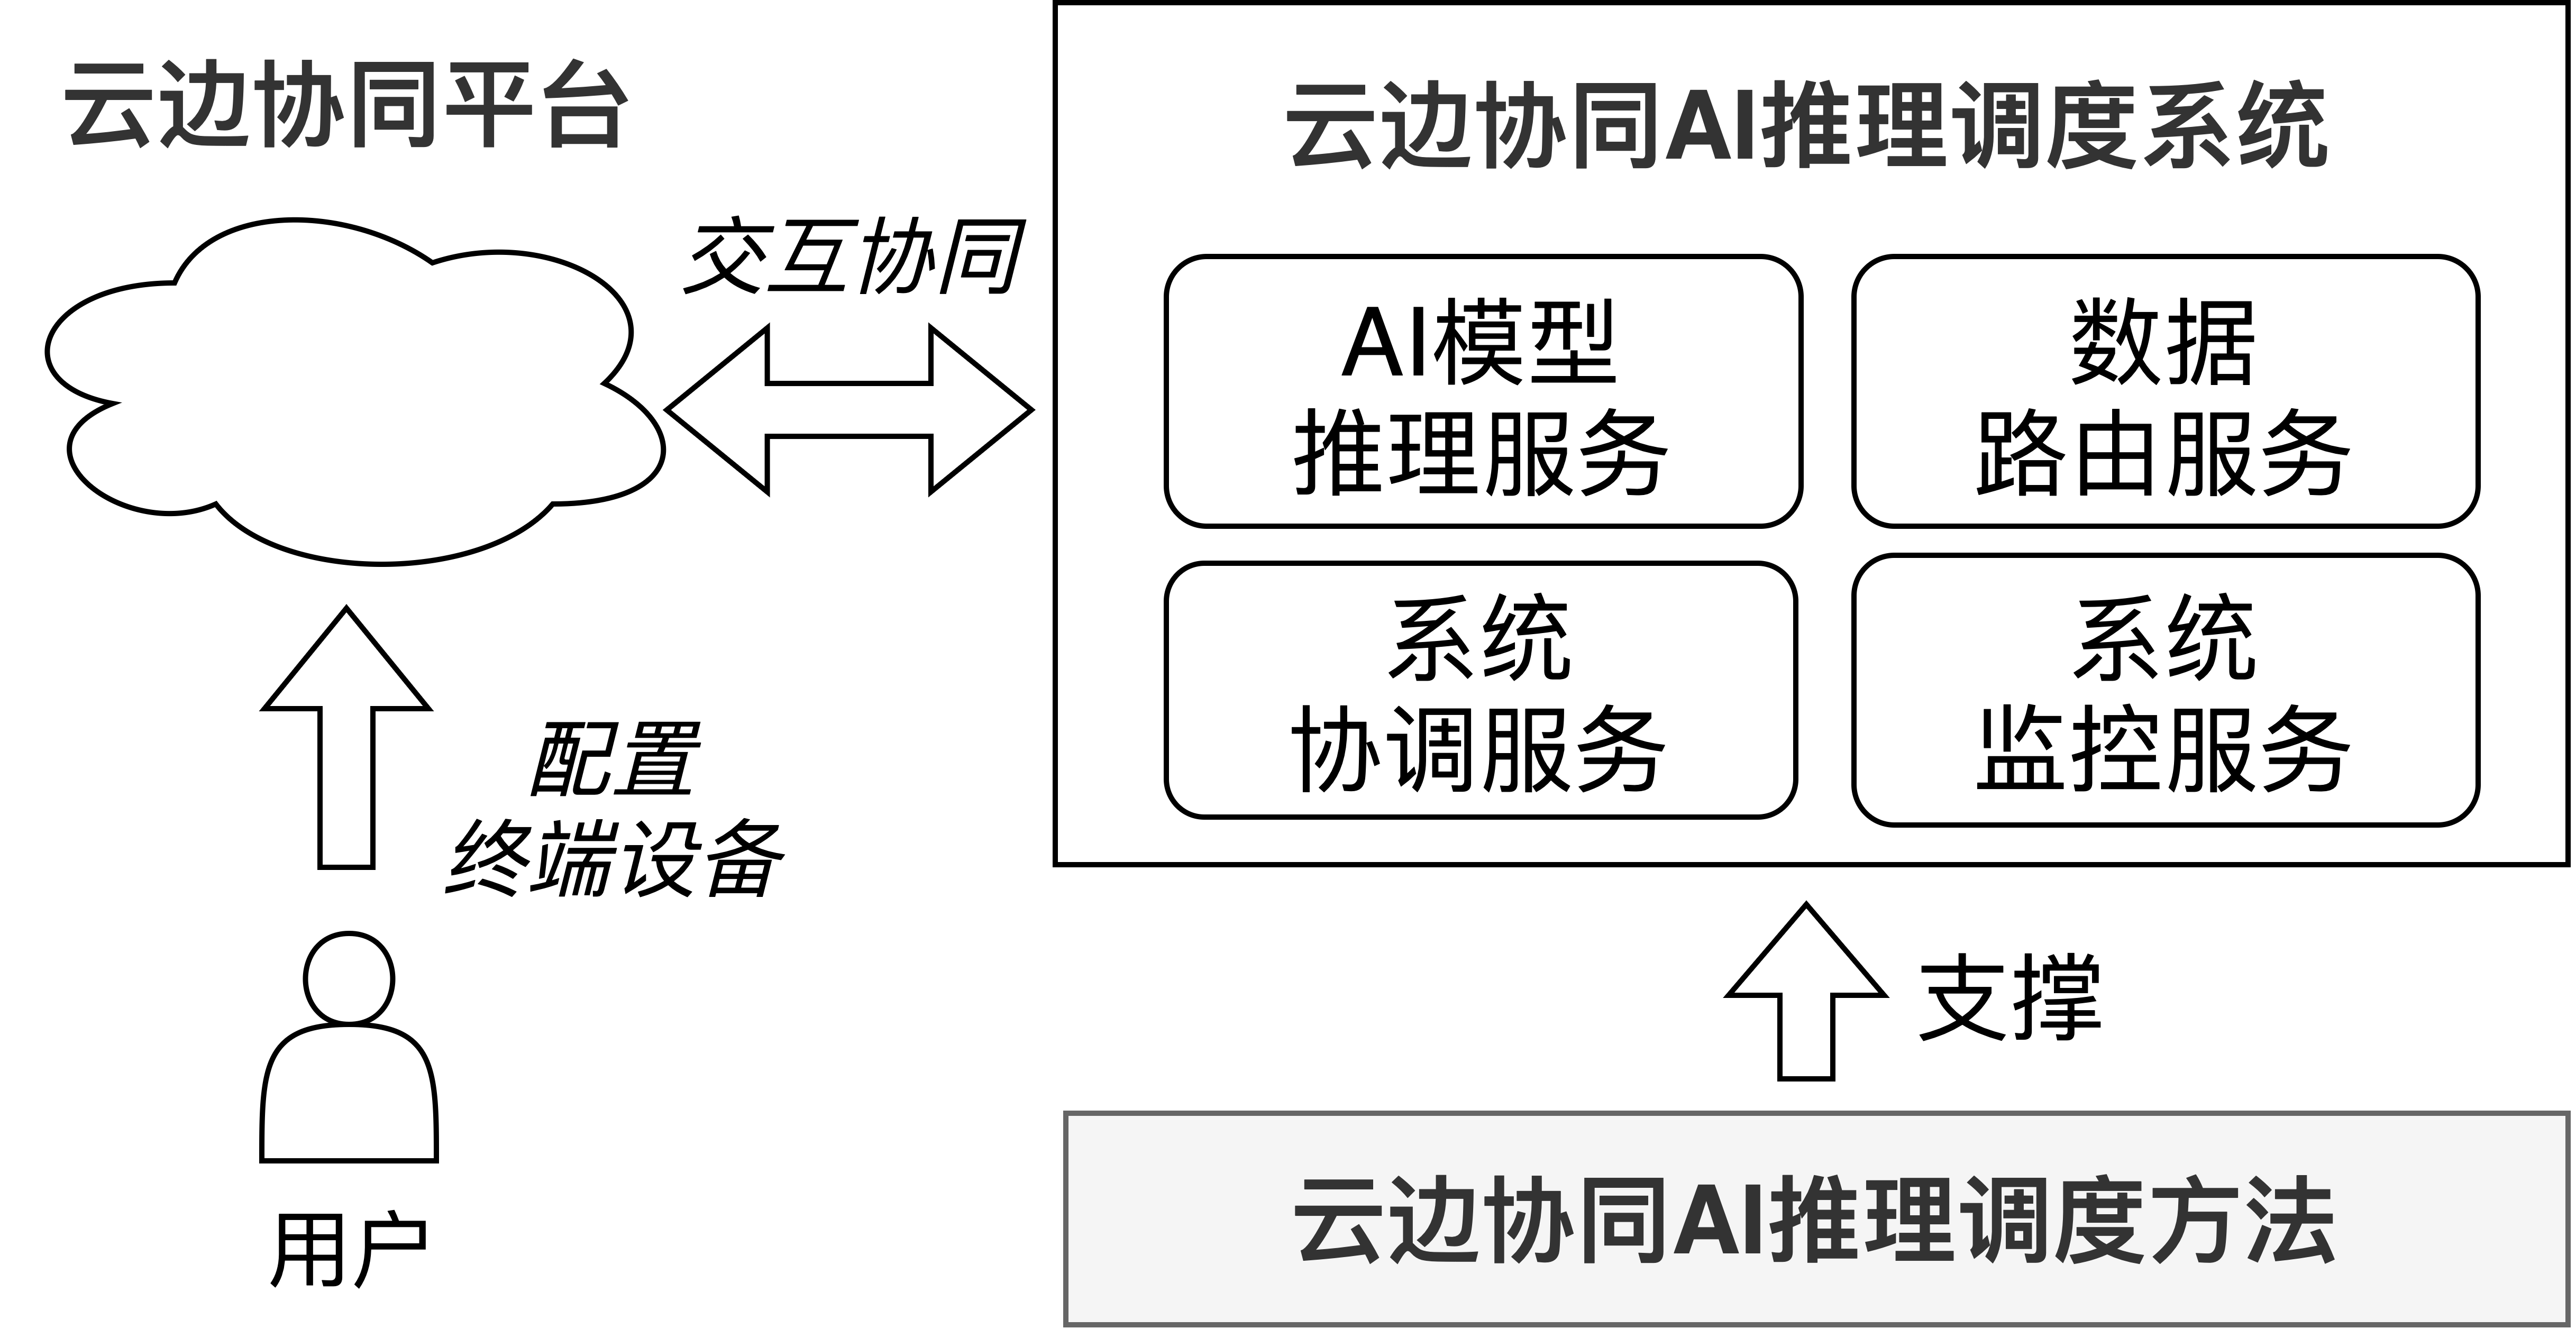
\includegraphics[width=0.7\linewidth]{pics/3-all.png}
  \caption{云边协同AI推理调度方案KEAS示意图}
  \label{fig:3-all}
\end{figure}

图\ref{fig:3-all}展示了本文提出的云边协同AI推理调度方案KEAS的整体架构。该方案涉及用户、云边协同平台、云边协同AI推理调度方法和系统等多个角色。在运行时,用户通过云边协同平台配置终端设备,这些设备会持续采集并生成流式时序数据。系统与云边协同平台保持实时交互,动态监测终端设备的状态信息,并结合边缘和云端的资源情况,动态调度流式时序数据的AI推理请求。通过边缘节点间的水平协作以及云端全局的垂直协同,该方案实现了资源的高效利用与任务的优化分配。

\begin{figure}[ht]
  \centering
  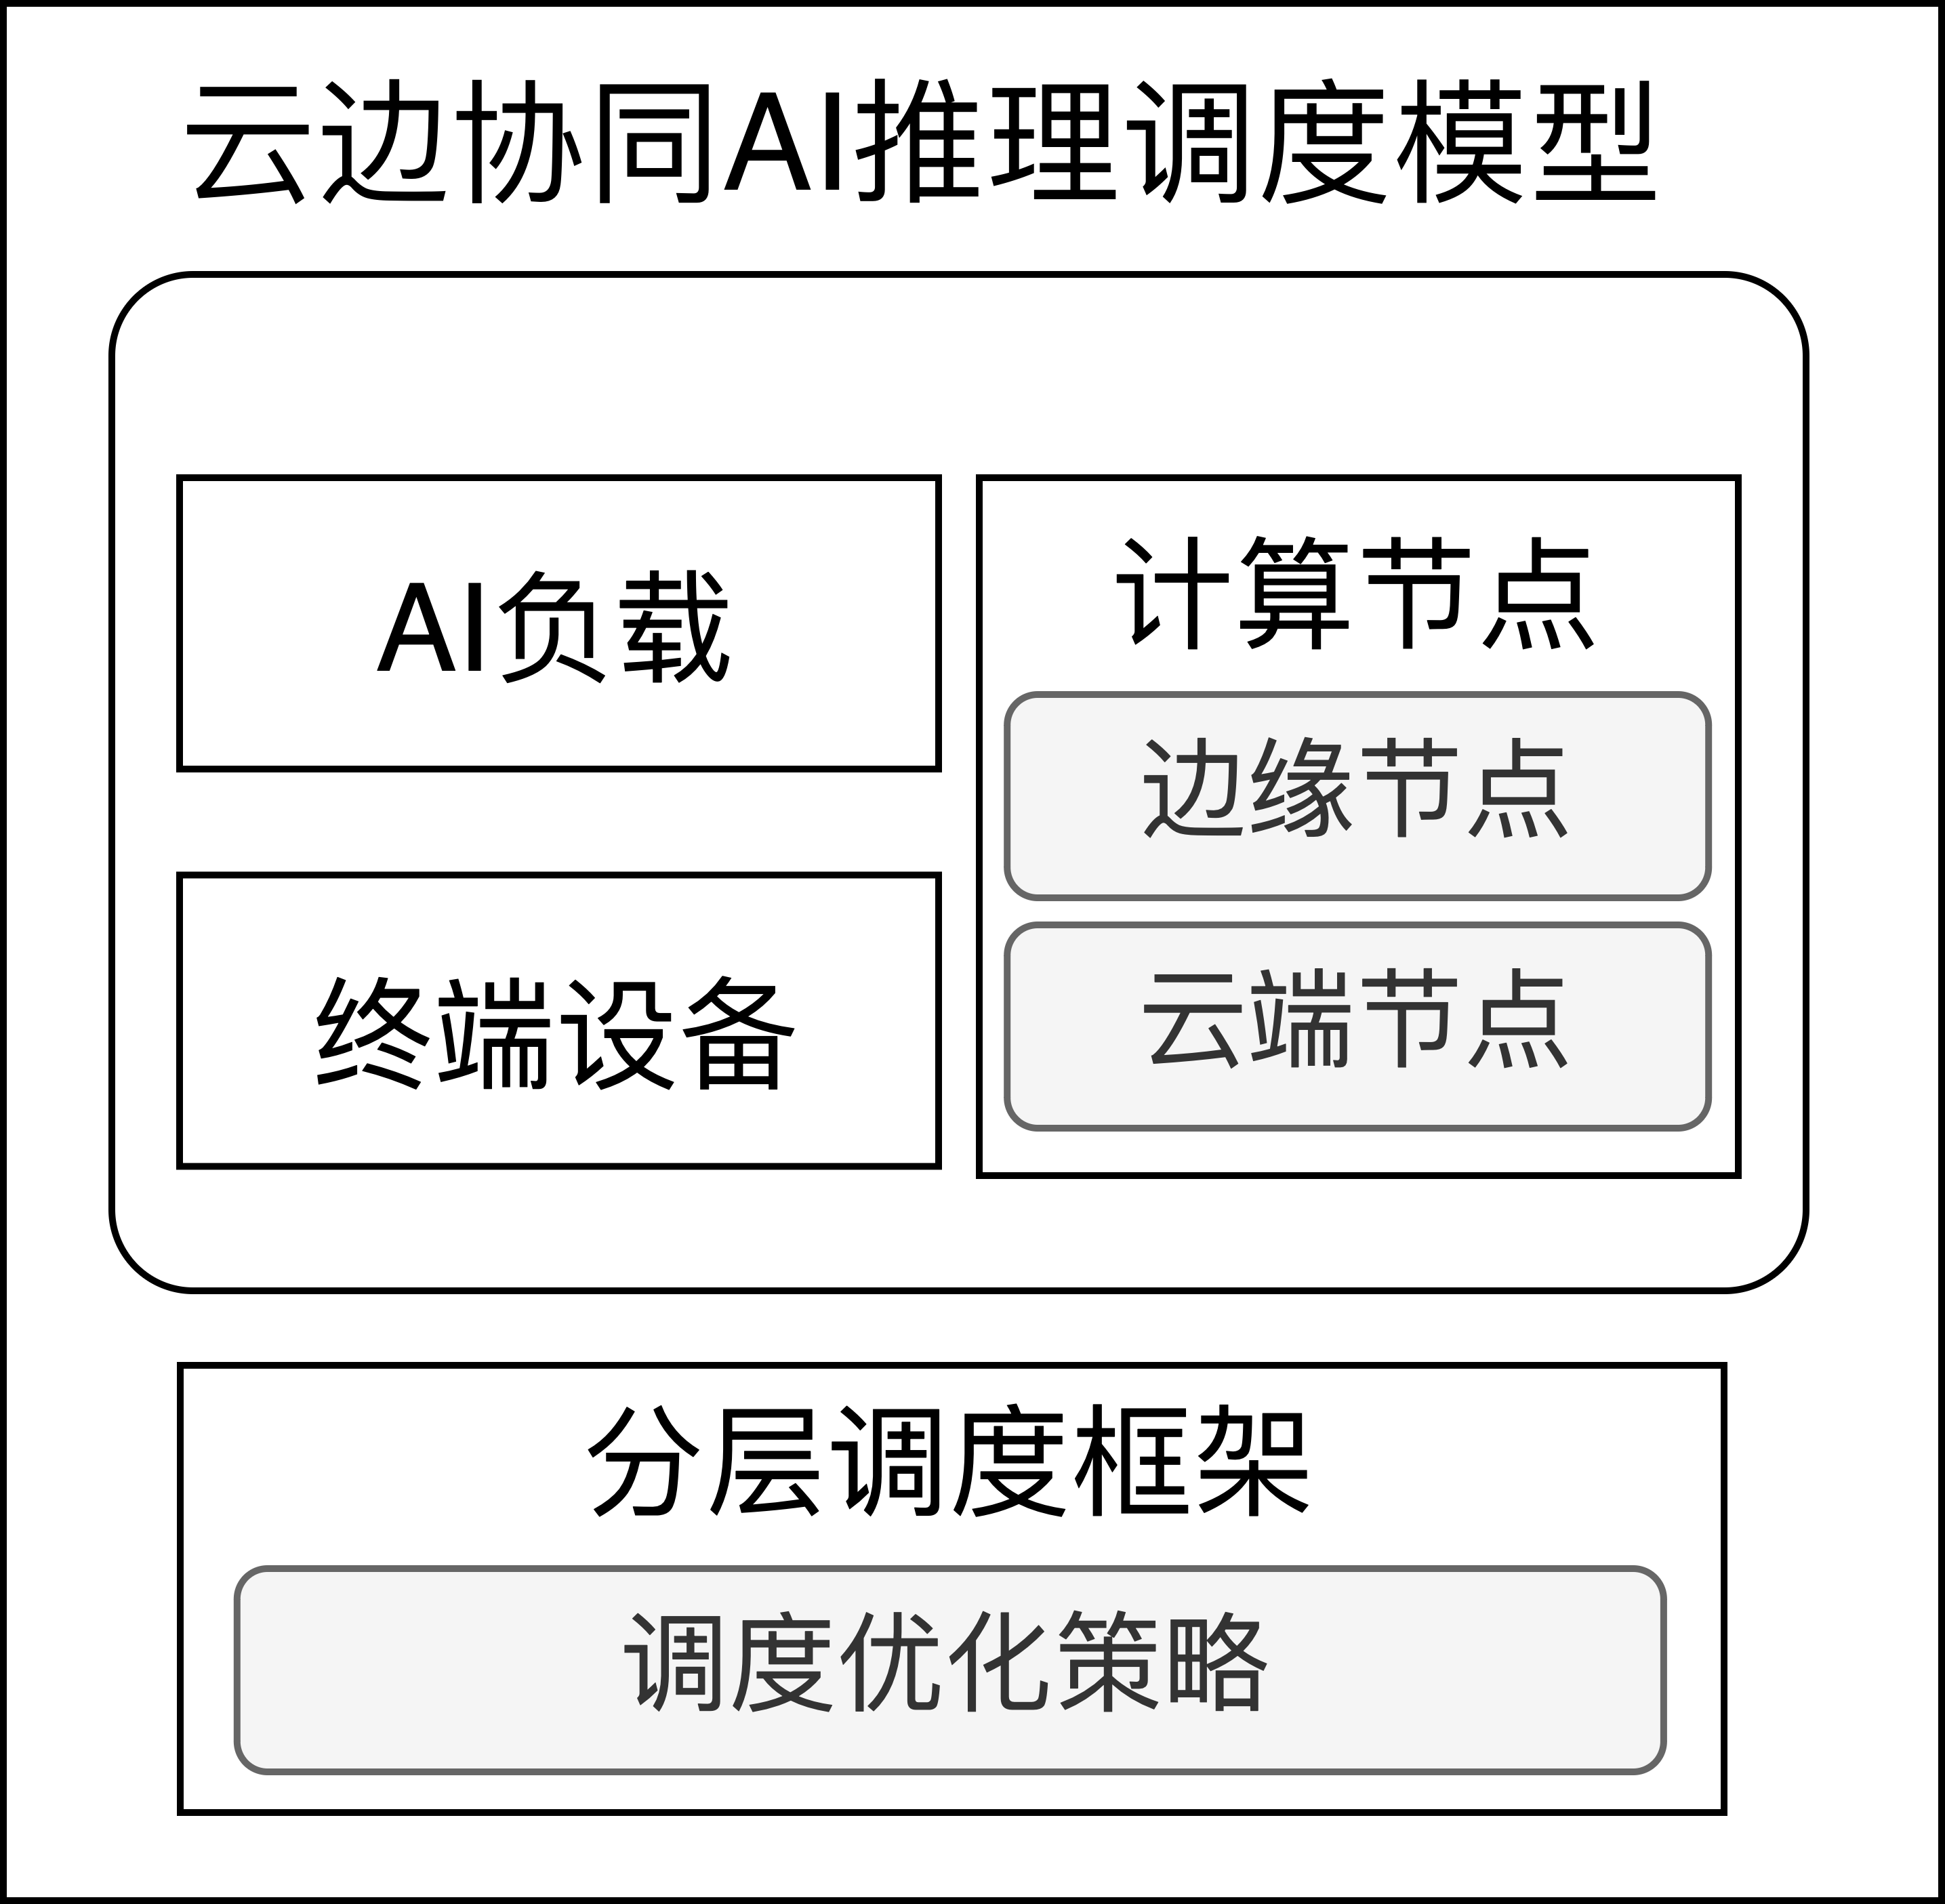
\includegraphics[width=0.4\linewidth]{pics/3-0架构.png}
  \caption{云边协同AI推理调度方法架构示意图}
  \label{fig:3-0arch}
\end{figure}

图\ref{fig:3-0arch}展示了方法的基本架构。该架构基于云边协同AI推理调度模型构建,清晰界定了云边平台的核心组件,包括终端设备、AI负载实例、计算节点、边缘集群及分层调度框架。同时,该模型详细定义了流式数据调度机制的关键要素,例如数据分流策略和各级调度器在运行时可见的状态信息等。基于此理论模型,本文提出了分层调度体系,其核心内容如下:

\begin{enumerate}
    \item \textbf{云边协同AI推理调度模型}:本文构建了形式化的云边协同AI推理调度模型,系统定义了终端设备、AI负载实例、计算节点等核心组件及其交互机制。通过引入计算队列状态感知和数据流驱动的动态调度框架,建立了覆盖边缘节点、集群到云端的多层级优化模型,为分层调度策略的设计奠定了理论基础。
    \item \textbf{云边协同AI推理分层调度策略}:本文提出分层调度架构。其中,本地调度策略以节点级资源最优分配为目标,通过动态调整分流比例优先保障直连设备服务质量,最小化跨节点传输开销;中间层次调度结合时延敏感度感知机制,构建多维度优先级队列,确保在满足时延约束的同时最大化集群内部资源利用率;云端全局调度策略构建跨域资源协调机制,采用最短任务先调度方法,减少碎片。
\end{enumerate}

\section{云边协同AI推理调度模型}

\subsection{模型定义}

云边协同的核心目标在于通过协调跨层级资源,以尽可能高效地满足物联网(IoT)设备的数据处理需求。为了实现IoT设备数据的高效采集,并提供灵活且高效的接入能力,现有框架通常借助抽象层来屏蔽底层硬件差异,进而为异构终端设备提供标准化的接入接口。例如,KubeEdge\cite{xiong2018extend}通过设备孪生(Device Twin)技术建立物理设备的数字镜像,支持基于标准MQTT协议接入工业传感器、智能摄像头等终端设备,其双向同步机制可保证设备状态与云端视图的一致性;Tango\cite{bagchi2017tango}则提出分层设备管理模型,通过边缘代理层(Edge Proxy)对Modbus、CAN总线等工业协议进行转换,为低功耗嵌入式设备提供资源虚拟化接口。若缺乏此类模块,开发人员则需自行实现设备协议解析、数据格式转换等底层适配逻辑,才能读取相关数据。

\begin{figure}[ht]
  \centering
  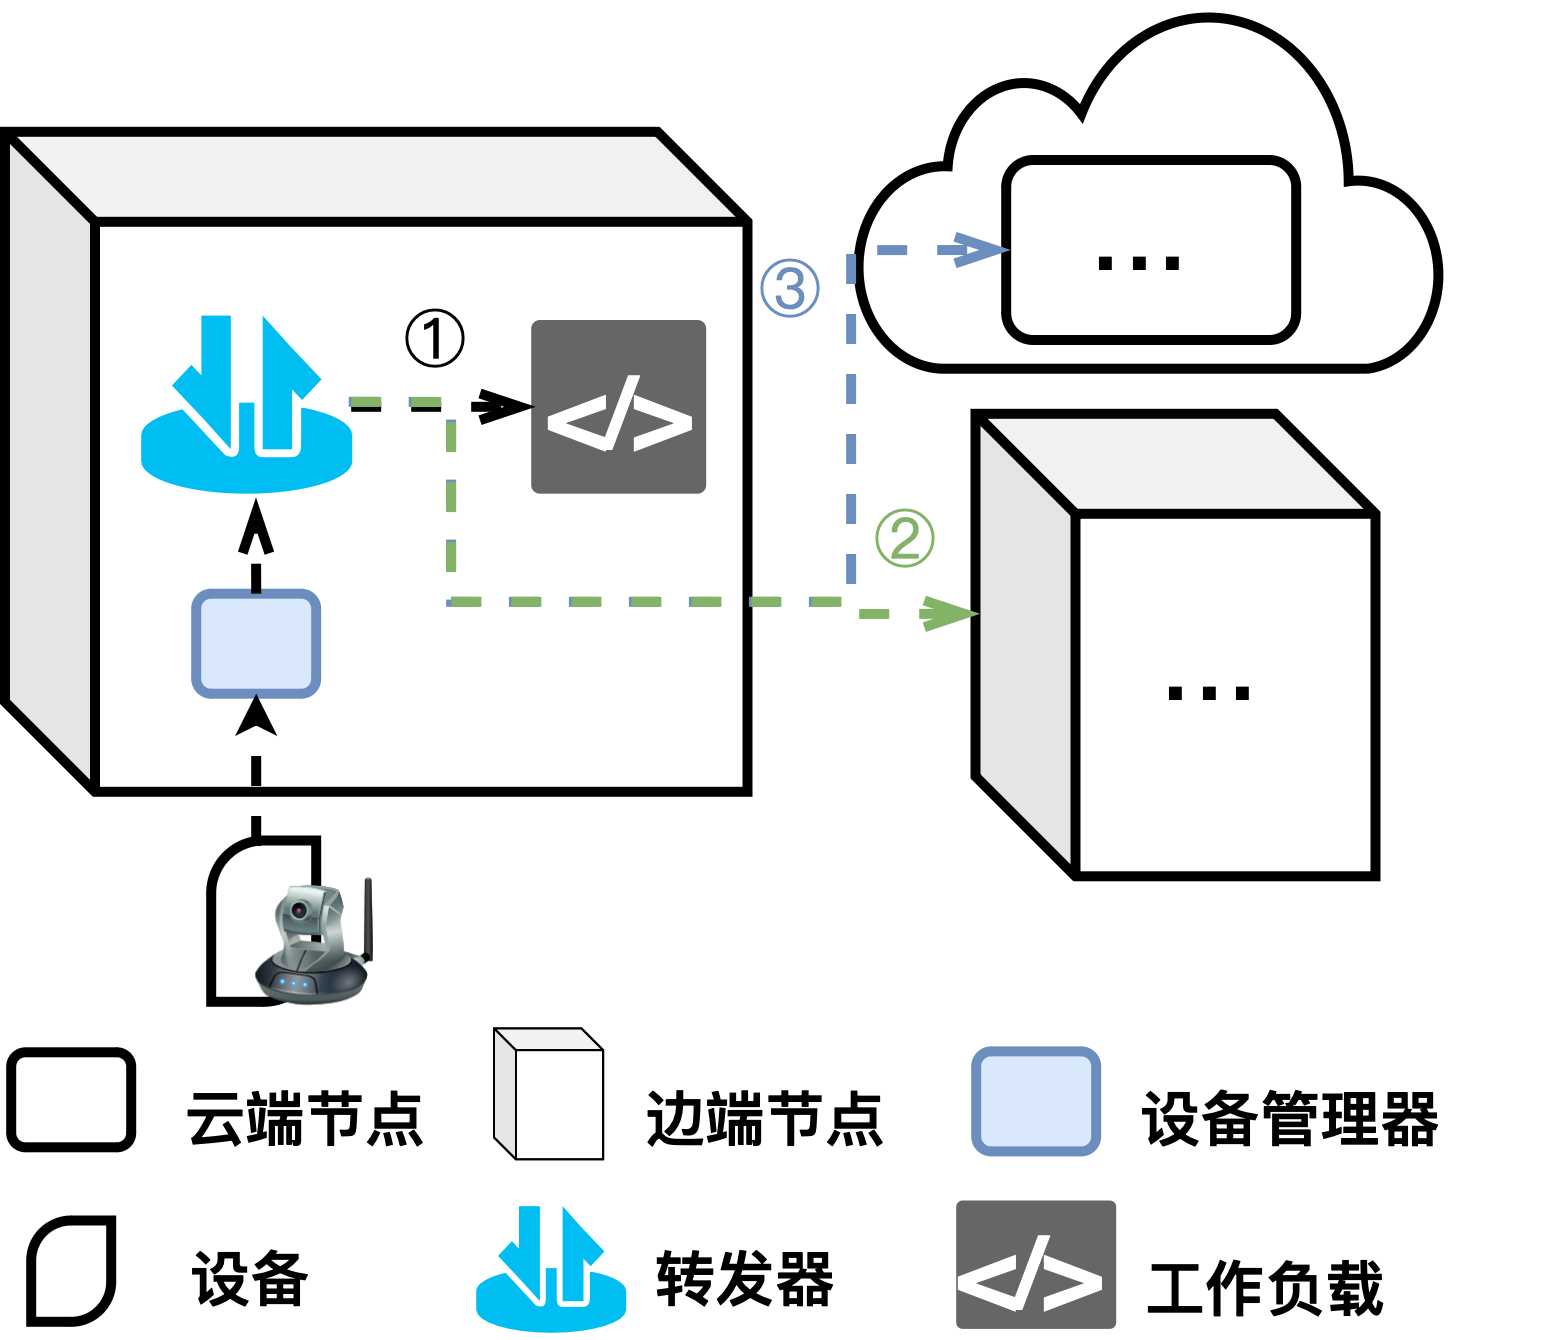
\includegraphics[width=0.5\linewidth]{pics/3-1流处理.png}
  \caption{流式数据调度与多级协作示意图}
  \label{fig:3-1flow}
\end{figure}

IoT设备产生的时序数据具有连续性强、时间敏感性高的特点,因此适合采用流处理范式进行实时处理\cite{de2018distributed,wang2020edge}。如图\ref{fig:3-1flow}所示,云边平台可根据负载状态,对于流式时序数据实现调度决策,既可以在本地边缘节点直接执行,也可以转发至其他边缘节点以实现水平方向的协作,或者依托云端全局视图实现云边节点间的跨层级垂直协作。目前,部分边端流处理框架已初步支持轻量级数据过滤与转发功能。例如,Kuiper\cite{ekuiper}通过SQL-like语法定义数据过滤规则,能够对原始数据进行实时过滤与简单转换,并将结果转发至其他节点,但尚未集成智能化的动态调度决策机制。这些引擎主要面向基于阈值的轻量级计算任务,尽管部分框架尝试适配AI推理功能,但尚未充分解决云边异构化环境下AI推理任务的部署问题,缺乏对深度学习框架版本冲突的兼容性保障以及跨架构硬件适配机制。

\begin{figure}[h]
  \centering
  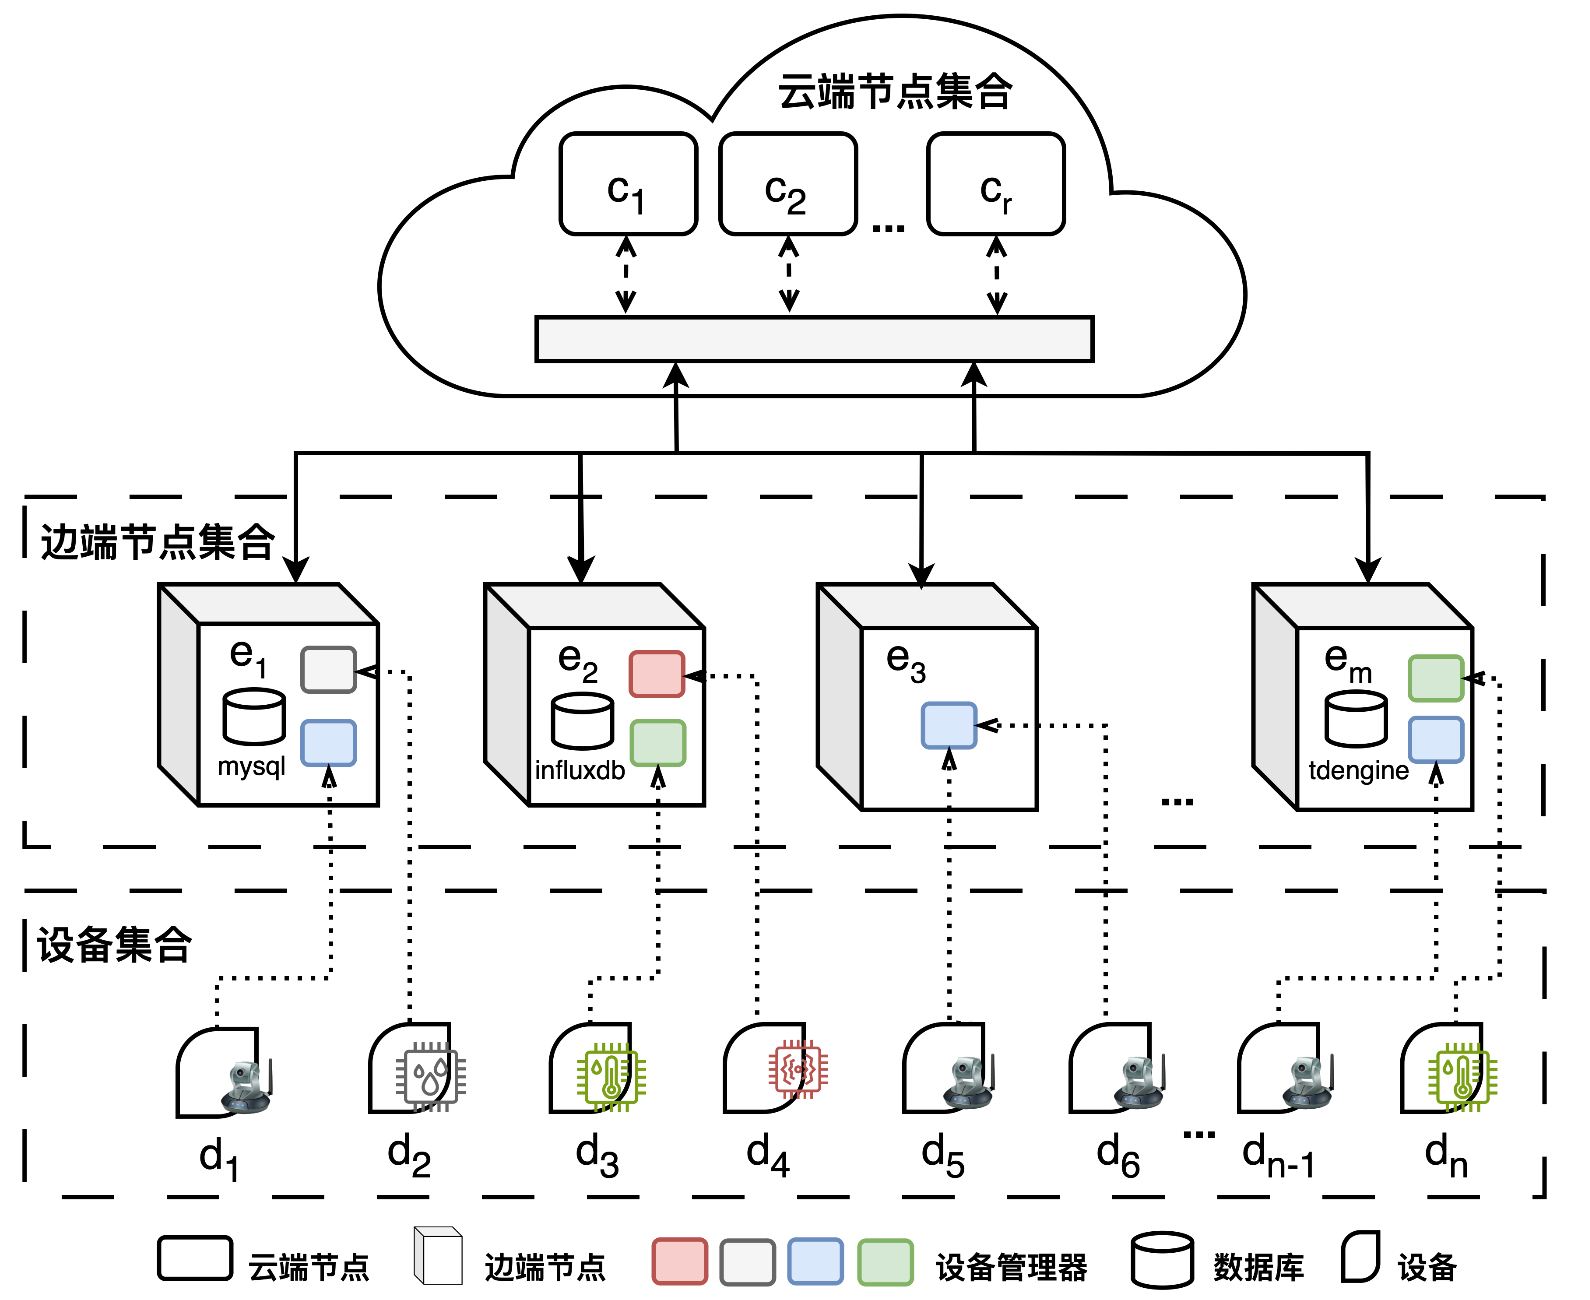
\includegraphics[width=0.9\linewidth]{pics/3-2模型架构.png}
  \caption{云边协同AI推理调度模型示意图}
  \label{fig:3-2model}
\end{figure}

针对上述架构特征与技术挑战,本文提出了一种云边协同AI推理调度模型,旨在系统性解决云边环境中的AI推理任务调度问题。该模型通过抽象任务特征与系统约束,构建了一个统一的调度框架,以支持多样化的AI应用场景。其核心目标包括:首先,明确云边环境的核心组成要素,包括计算节点、网络拓扑、AI负载以及终端设备,为模型的设计提供清晰的结构化基础;其次,形式化描述AI推理过程中的关键开销,包括计算开销、通信开销等,从而为后续的调度算法实现奠定坚实的理论基础。

下面给出云边协同AI推理调度模型的形式化定义:

\begin{definition}[云边协同AI推理调度模型]
云边协同 AI 负载调度模型可表示为一个5元组:
\end{definition}

$$
\mathcal{M} = (\mathcal{D}, \mathcal{E}, \mathcal{C}, \mathcal{L}, \mathcal{B})
$$

其中:

\begin{itemize}
    \item $\mathcal{D} = \{d_i\}_{i=1}^n$ 表示终端设备集合,其中每个终端设备$d_i$用于物联网数据采集,具体定义详见定义\ref{def:device}。
    \item $\mathcal{E} = \{e_j\}_{j=1}^m$ 表示边缘节点集合,每个节点$e_j$具有有限计算资源,部署在网络边缘靠近终端设备的位置,具有低时延响应能力。
    \item $\mathcal{C} = \{c_q\}_{q=1}^r$ 表示云端节点集合,每个节点$c_q$配备高性能计算资源,适用于计算密集的大规模AI推理或模型训练。
    \item $\mathcal{L} = \{\ell_s\}_{s=1}^u$ 表示AI负载实例集合,其中每个AI负载实例$\ell_s$负责处理终端设备产生的实时流数据并执行推理任务,具体定义详见定义\ref{def:aimodel}。
    \item $\mathcal{B} \in \mathbb{R}^{\mu \times \mu}$ 为带宽矩阵,其中$\mu=m+r$,表示云边环境下的所有节点,元素 $b_{pq}$ 表示节点 $p$ 到节点 $q$ 的有效带宽。
\end{itemize}

为了更清晰地描述模型的动态运行特性,本文将云边平台的运行时间划分为一系列等长时间窗 $\{t_\omega\}_{\omega=1}^\infty$。其中,第 $\omega$ 个调度时间窗定义为 $t_\omega = [\tau_\omega, \tau_\omega + \Delta t)$,$\Delta t$ 表示时间窗的长度参数。在此基础上,后续章节将进一步展开对计算节点、终端设备、AI 负载的详细分析。

\subsubsection{计算节点}

在云边协同计算架构中,计算节点作为任务处理和资源分配的核心实体,承担着数据处理、存储以及通信的关键职能。计算节点集合$\mathcal{V} = \mathcal{E} \cup \mathcal{C}$涵盖边缘节点集合$\mathcal{E}$与云端节点集合$\mathcal{C}$,其中总共包含$\mu=m+r$个计算节点。由于云边环境中的节点具有异构化的资源供给和硬件架构特性,为了实现高效的 AI 负载部署,需要对每个节点的资源供给能力、硬件架构特性和计算能力进行量化分析。这种量化过程能够为任务调度和资源优化提供科学依据,从而提升整体系统的性能与效率。

下面给出计算节点的形式化定义:

\begin{definition}[计算节点]
\label{def:node}
计算节点 $v_j \in \mathcal{V}$ 可表示为一个 3 元组:
\end{definition}

$$
v_j = (R_j,\, Arch_j,\, Perf_j)
$$

其中:
\begin{itemize}
    \item $R_j = \{r^{k}_j\}_{k=1}^w$ 表示资源供给向量,其中 $r^{(k)}_j \in \mathbb{R}^+$ 表示第 $k$ 类资源总量。
    \item $Arch_j \in \mathbb{H}$ 表示硬件架构,$\mathbb{H}$ 为硬件架构类型枚举集。
    \item $Perf_j \in \mathbb{R}^+$ 表示计算性能,单位为每秒浮点运算次数(FLOPS)。
\end{itemize}

\subsubsection{终端设备}

在物联网架构下,终端设备作为数据采集的核心单元,其行为特性可以从静态属性和动态数据采集两个维度进行刻画。静态属性描述了设备的固有能力与接口规范,这些属性在设计阶段确定,通常不可更改,能够表征设备类型;而动态数据采集则关注设备运行时的数据生成过程,包括采样频率、传输速率等特性,这些特性随设备的工作状态而波动,反映着设备实时交互与响应的能力。

下面给出终端设备的形式化定义:

\begin{definition}[终端设备]
\label{def:device}
终端设备 $d_i \in \mathcal{D}$ 可表示为一个 2 元组:
\end{definition}

$$
d_i = (\Omega_\beta, g_\beta)
$$

其中:
\begin{itemize}
    \item $\Omega_\beta = (X^{(k)}_\beta)_{k=1}^{\zeta}$ 表示静态属性集合($\zeta \in \mathbb{N}^+$ 为属性维度),表征设备的物理特性。
    \item $g_\beta(t)$ 表示瞬时数据采集频率函数,需满足 Lipschitz 连续条件:
        \begin{equation}
        \exists K_\beta > 0,\ \forall t_1, t_2 \in \mathbb{R},\ |g_\beta(t_2) - g_\beta(t_1)| \leq K_\beta |t_2 - t_1|
        \end{equation}
        其中 $K_\beta$ 表示设备物理特性决定的最大调节速率。
\end{itemize}

终端设备的静态属性体现了显著的类型特异性,这种特异性源于设备在功能设计和物理实现上的差异。例如,视觉设备的静态属性通常包括分辨率、位深度、压缩算法及总线配置等量化参数;温度传感器则包含量程范围和测量精度等物理特性参数。为简化论述,本文假设初始场景中所有终端设备属于单一类型,该假设可通过服务发现机制扩展至多设备场景。

这些静态属性不仅表征了设备的基础能力,还为数据量计算提供了关键依据。以视觉设备为例,其单帧数据量可通过分辨率与位深度的乘积初步估算,并结合压缩率修正得出精确值。本文采用$\varsigma_\beta \in \mathbb{R}^+$ 表示单次数据采集量,通过标准化转换函数计算:

\begin{equation}
\varsigma_\beta = \varphi(\Phi_\beta) = \prod_{k=1}^{\zeta} f_k(X^{(k)}_\beta)
\end{equation}

其中 $f_k: \mathcal{P} \to \mathbb{R}^+$ 为预定义的属性量化函数。进一步地,终端设备 $d_i$ 的瞬时数据采集流量 $G_i(t)$ 由瞬时数据采集频率 $g_i(t)$ 和单次采集量 $\varsigma_\beta$ 共同决定,具体表达式为:

\begin{equation}
G_i(t) = g_i(t) \cdot \varsigma_\beta
\end{equation}

\begin{figure}[h]
  \centering
  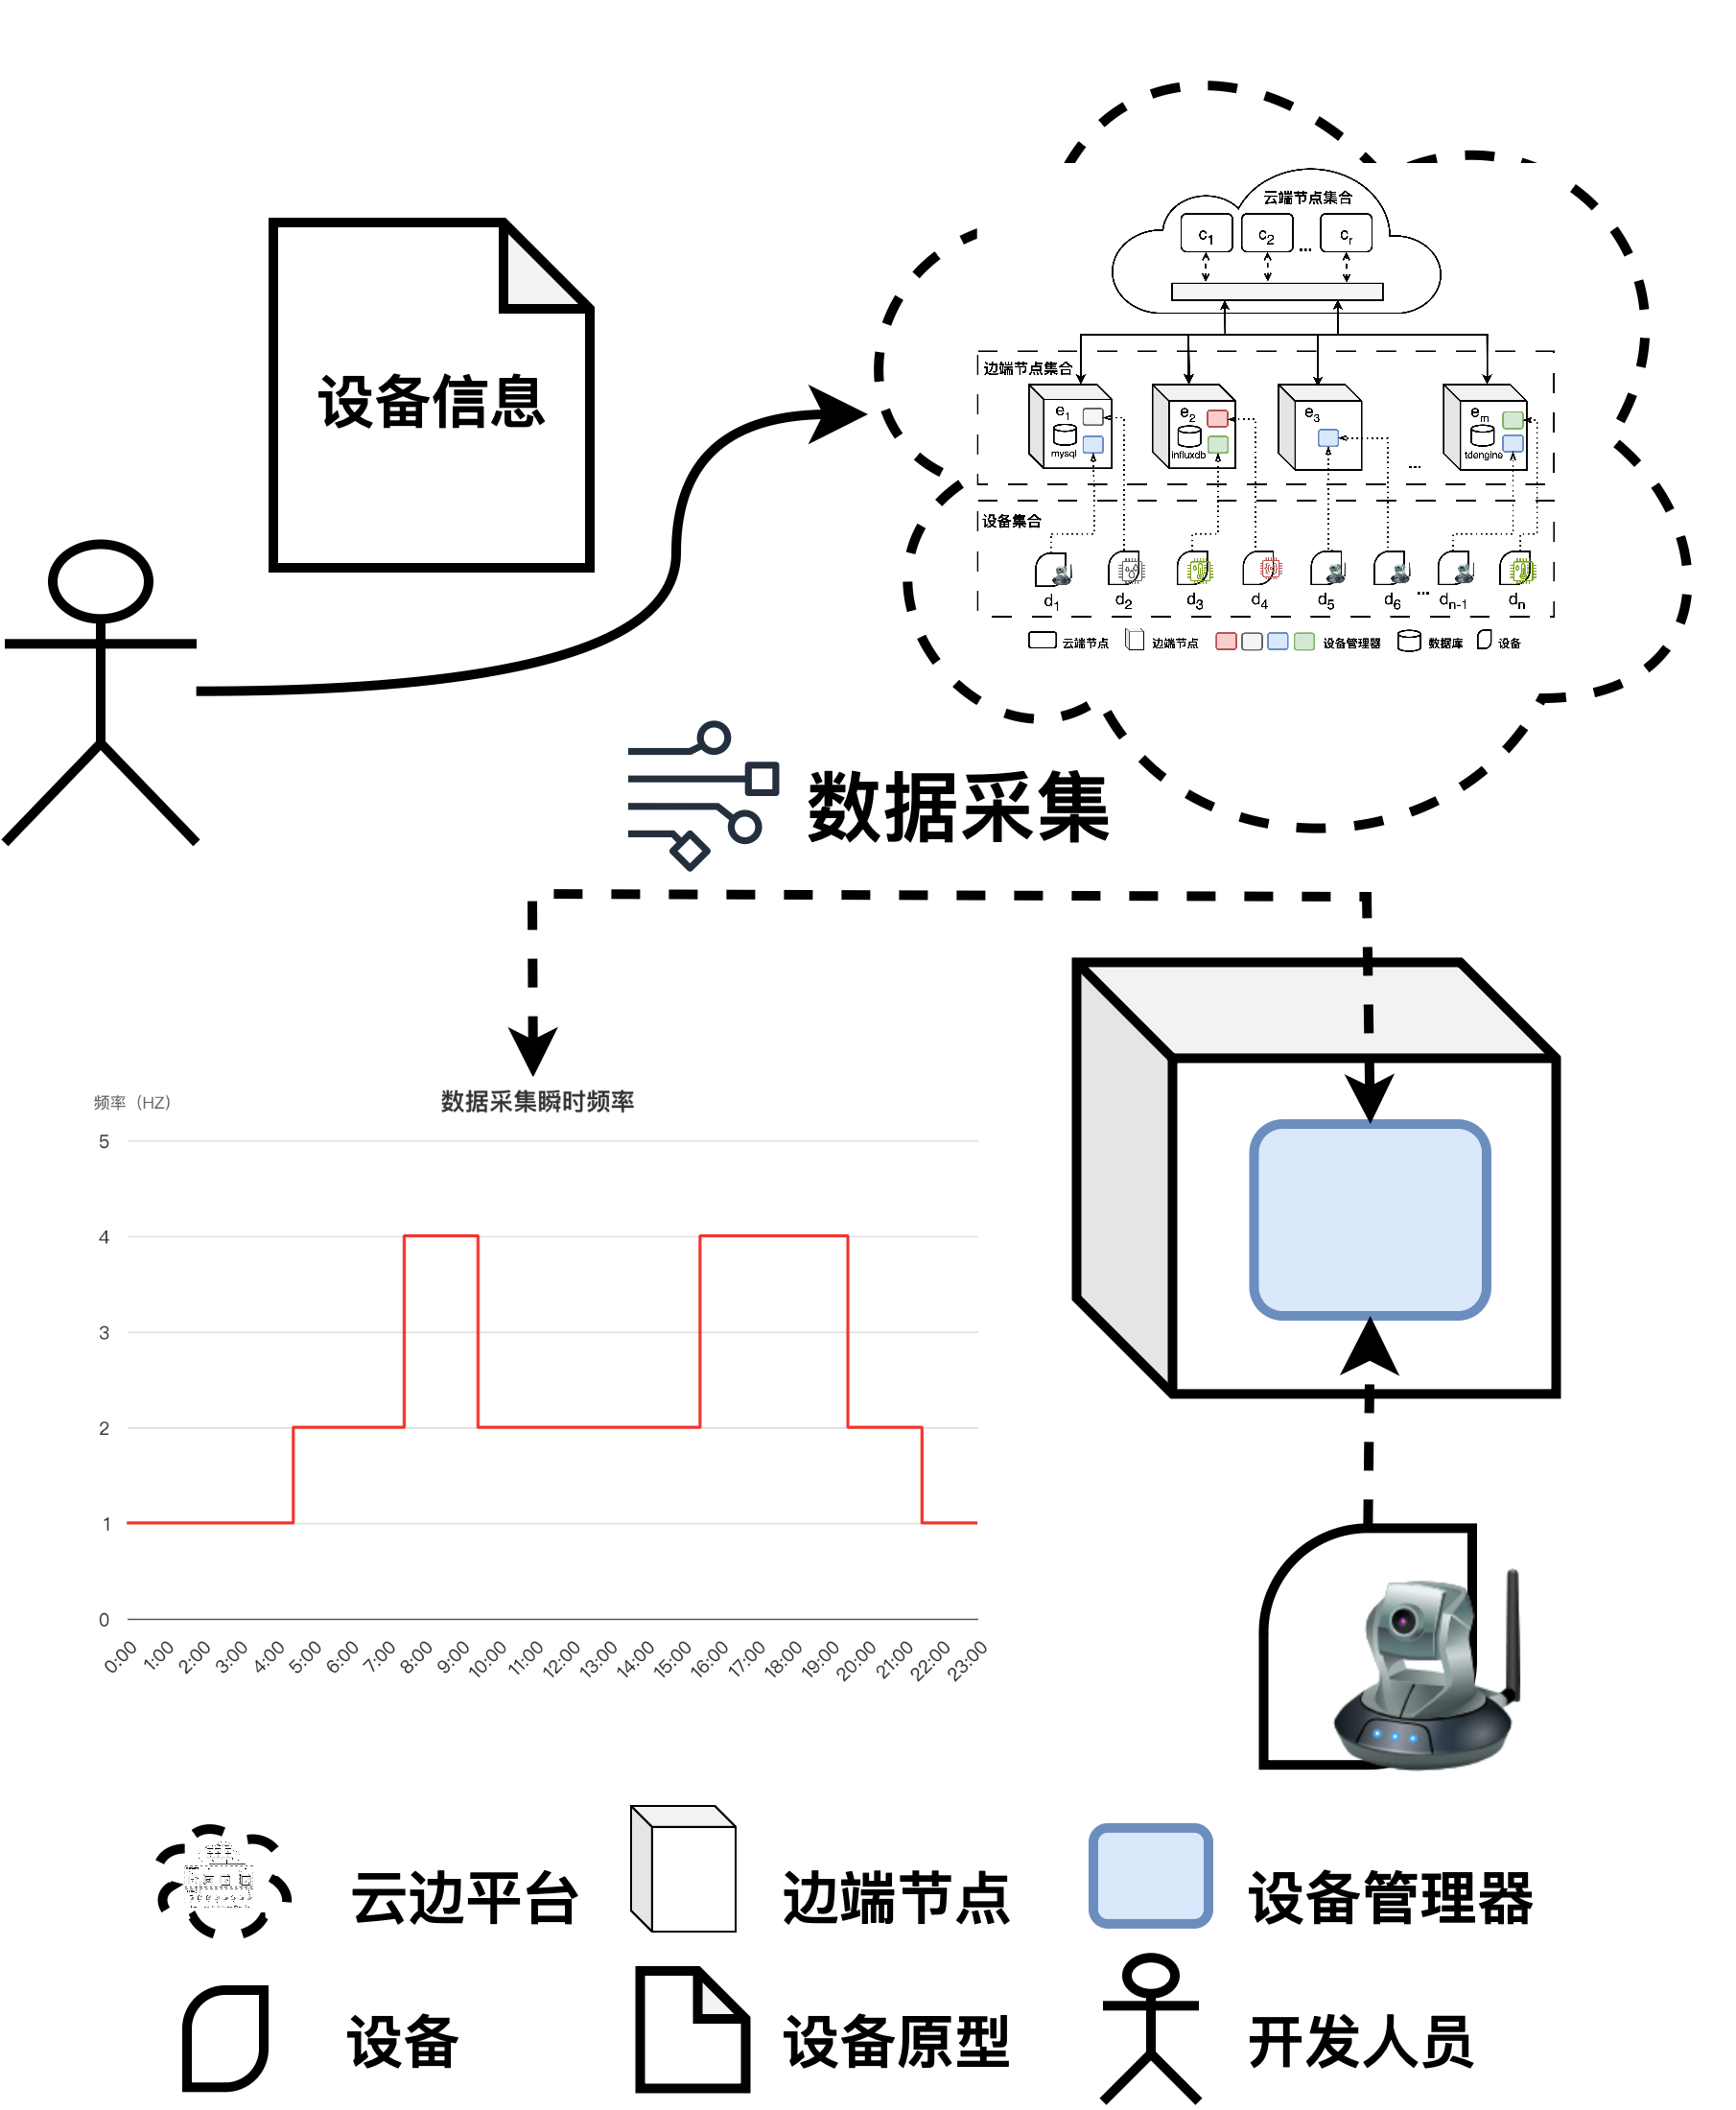
\includegraphics[width=0.55\linewidth]{pics/3-3设备模型.png}
  \caption{设备数据采集流程图}
  \label{fig:3-3device}
\end{figure}

根据上述定义,终端设备的数据采集过程可以被完整抽象,如图 \ref{fig:3-3device} 所示。首先,开发人员将设备静态属性注册至云边平台。在此过程中,云边平台通过解析设备原型的静态属性提取出设备的关键能力描述,并生成与该设备对应的设备管理器。设备管理器不仅负责存储和维护设备的静态属性,还用于动态调整和管理设备运行时的行为特性。在设备注册完成后,利用预定义的标准化转换函数 $f_k$ 对静态属性进行量化,从而计算每次数据传输的具体量 $\varsigma_\beta = \varphi(\Phi_\beta)$。这一量化结果为后续的数据采集流量计算提供了基础依据。与此同时,设备管理器调整瞬时数据采集频率函数$g_\beta(t)$,以满足不同时段对设备数据采集的需求。

\subsubsection{AI 负载实例}

在云边协同的推理场景中,AI负载实例的核心功能是处理终端设备产生的实时流数据。终端设备(如传感器、摄像头等)持续生成大量高时效性和多样性的实时数据流。然而,这些原始数据通常需要经过预处理才能被AI负载实例有效利用。由于不同类型的终端设备生成的数据格式和特性各异,其预处理需求也各不相同。例如,视觉设备可能需要图像压缩或格式转换,而传感器数据可能需要滤波或归一化处理。如图\ref{fig:3-4aiload}所示,预处理逻辑的部署位置具有灵活性:既可以在设备管理器采集数据时实时完成,也可以在AI推理实例中进行处理。此外,云边环境中的数据转发器能够根据实际需求,选择性地传输已预处理的结构化数据或原始数据,从而在保持数据时效性的同时,为不同场景提供灵活的处理方案。

\begin{figure}[h]
  \centering
  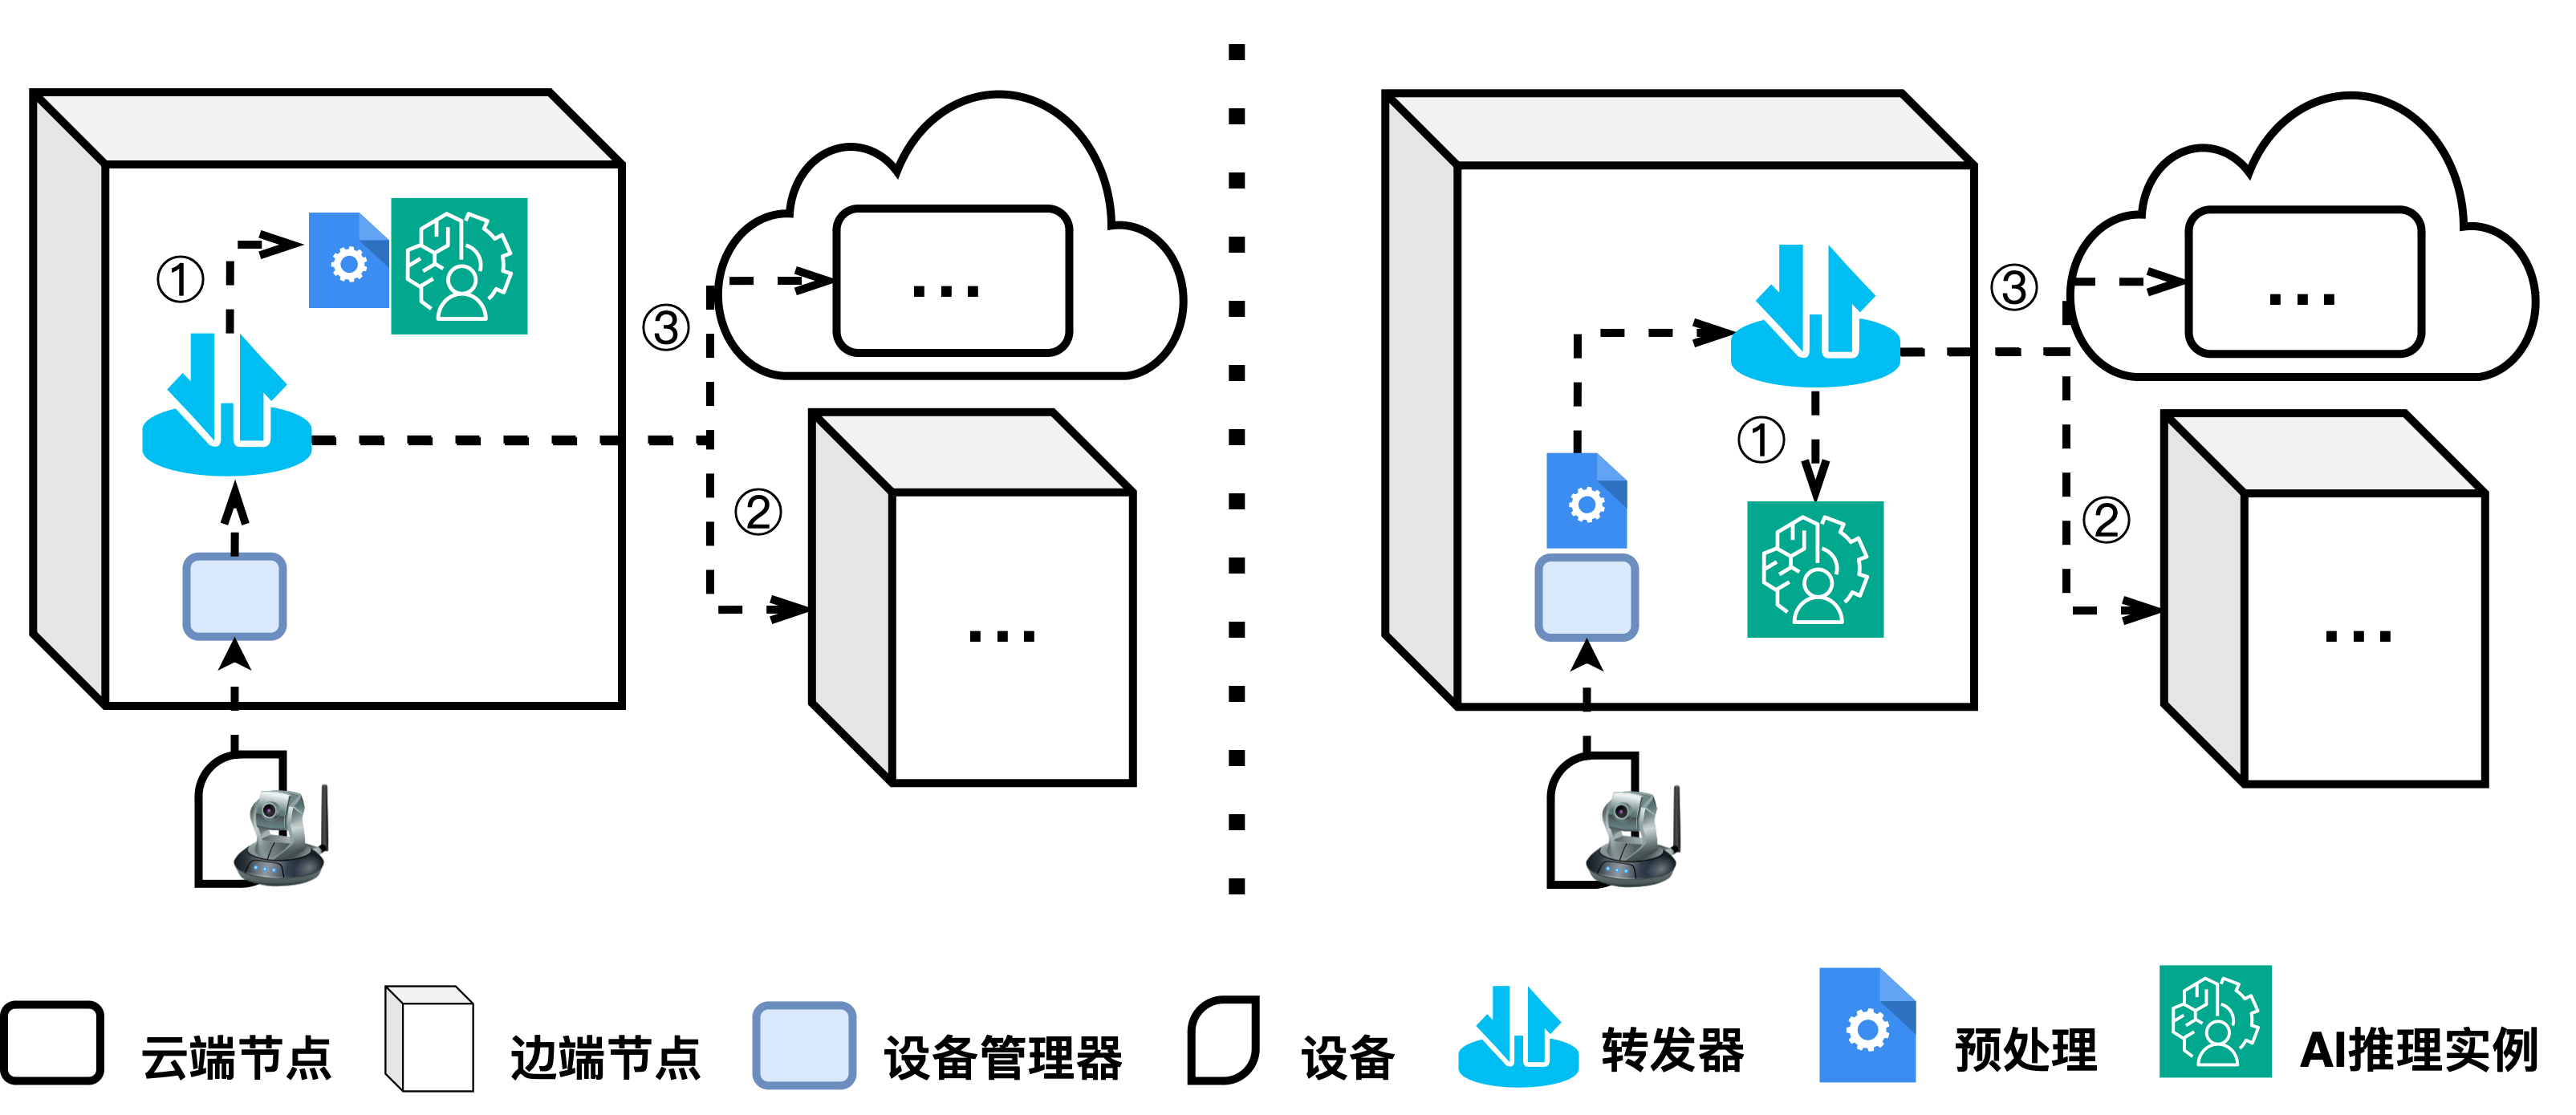
\includegraphics[width=0.9\linewidth]{pics/3-4AI负载.png}
  \caption{云边环境下AI负载的端到端处理流程}
  \label{fig:3-4aiload}
\end{figure}

当经过预处理的数据传递至AI负载实例后,推理过程即可在适配的计算节点上执行。然而,AI负载实例对不同节点的适配性存在显著差异,这主要体现在深度学习框架、硬件指令集依赖与推理资源需求等方面。首先,AI模型通常在特定框架及其版本下开发,而不同计算节点可能未安装所需的框架或版本。此外,许多框架的版本与其对硬件指令集的支持深度绑定,这种绑定关系直接影响模型的部署和运行效率。例如,当前主流框架(如TensorFlow)的最新版本通常默认启用AVX2指令集优化,以大幅提升张量运算性能。然而,在将其部署到不支持AVX2指令的边缘节点时,则需要通过重新编译框架源码或降级至兼容版本来实现正常运行。即便目标节点具备相应的硬件指令集,不同架构(如x86与ARM)对同一指令集的优化程度也可能导致运行效率的显著差异\cite{ren2019performance}。这种硬件架构的异构性要求在部署AI负载时,必须明确其对指令集和架构的具体需求。

其次,资源需求是影响AI负载适配性的另一关键因素。许多大型深度学习模型在设计之初便针对GPU等高性能加速器进行优化,依赖于GPU的大规模并行计算能力。然而,在资源受限的边缘节点上,可能缺乏GPU或其他专用加速器,导致模型无法运行或运行效率低下。同时,为了充分利用节点的计算能力,不同的AI负载实例会根据节点性能配置相应的批处理规模。例如,在高性能云端节点上可以采用较大的批处理规模以提高吞吐量,而在资源受限的边缘节点上则需降低批处理规模以避免资源过载。

上述问题表明,异构环境下的AI负载部署面临诸多挑战,包括框架兼容性、指令集支持以及资源适配性等复杂因素。为了解决这些问题,我们需要形式化定义AI负载实例的关键属性,以量化其对框架、硬件架构和资源的需求,并评估其在不同节点上的适配性。这种形式化的描述不仅有助于优化任务调度策略,还能显著提升系统在动态异构环境中的整体性能。

\begin{definition}[AI负载实例] 
\label{def:aimodel}
AI负载实例$\ell_s \in \mathcal{L}$ 可表示为一个 5 元组:
\end{definition}

$$
\ell_s = (\mathcal{F}_s,\, \mathcal{A}_s,\, \mathcal{R}_s,\, \gamma_s,\, \varpi_s)
$$

其中:
\begin{itemize}
    \item $\mathcal{F}_s \in \mathbb{S}$ 表示支持的深度学习框架,$\mathbb{S}$为云边平台支持的深度学习框架枚举集。
    \item $\mathcal{A}_s \subseteq \mathbb{H}$ 表示硬件架构需求集合,$\mathbb{H}$为硬件架构类型枚举集。
    \item $\mathcal{R}_s = \{r^{(k)}_s\}_{k=1}^w$ 表示资源需求向量,其中$r^{(k)}_s \in \mathbb{R}^+$对应第$k$类资源的最小需求。
    \item $batch_s \in \mathbb{Z}^+$ 表示批处理规模,满足$batch_s \leq \lfloor \frac{R_s}{\delta_s} \rfloor$,其中$R_s$为设备内存容量,$\delta_s$为单样本内存占用量。
    \item $\varpi_s \in \mathbb{R}^+$ 表示单次推理运算量,单位为浮点运算次数(FLOPs)。
\end{itemize}

在明确了AI负载实例的形式化定义后,AI 负载实例 $\ell_s$ 需要与目标节点 $v_q$ 的资源供给和硬件架构相匹配。具体而言,需满足以下条件:

\begin{equation}
\rho_q \geq \mathcal{R}_s, \quad \alpha_q \in \mathcal{A}_s, \quad \forall v_q \in \mathcal{V}
\end{equation}

其中,$\rho_{q}$ 和 $\mathcal{R}_s$ 分别表示节点 $v_q$ 的资源供给向量和负载实例 $\ell_s$ 的资源需求向量;$\alpha_q$ 和 $\mathcal{A}_s$ 分别表示节点 $v_q$ 的硬件架构和负载实例 $\ell_s$ 的硬件架构需求。

基于对AI负载实例与计算节点的形式化定义,本文构建推理时间预测函数$\text{Latency}_{\text{inf}}$来量化负载实例$\ell_s$在节点$v_j$上的单次推理延迟,该函数可表示为:

\begin{equation}
\text{Latency}_{\text{inf}}(\ell_s, v_j)= \frac{\varpi_s}{Perf_j}
\end{equation}

其中, $\varpi_s$ 为单次推理运算量,$Perf_j$为节点$v_j$的计算性能。

对于任意时间窗$t_\omega = [\tau_\omega, \tau_\omega + \Delta t)$,节点$v_j$可承载的AI负载实例$\ell_s$的最大吞吐量$Q(\ell_s, v_j, t_\omega)$可由下式计算:

\begin{equation}
Q(\ell_s, v_j, t_\omega) = \left\lfloor \frac{\Delta t}{\text{Latency}_{\text{inf}}(\ell_s, v_j)} \right\rfloor \cdot batch_s
\end{equation}

该指标$Q(\ell_s, v_j, t_\omega)$表示节点$v_j$在时间窗$t_\omega$内对负载$\ell_s$的最大服务容量,是衡量节点资源利用率和服务能力的重要参考。在实际部署过程中,这一指标由节点资源监控模块动态维护,并作为协同调度器决策过程的核心输入之一。调度器需确保分配至节点$v_j$的负载实例$\ell_s$的请求速率不超过其最大吞吐量$Q(\ell_s, v_j, t_\omega)$,从而避免因计算资源过载而导致的排队延迟或任务失败。

\subsection{数据流驱动的动态调度机制}

在云边协同环境中,终端设备产生的实时流数据是整个系统调度的核心驱动因素。根据定义3.3中终端设备的形式化描述,可以推导出在时间窗$t_\omega = [\tau_\omega, \tau_\omega + \Delta t)$内,设备 $d_i$ 的数据采集总量为$g_i^{t_\omega} = \int_{\tau_\omega}^{\tau_\omega + \Delta t} g_i(t) \, dt$,其中$g_i(t)$ 表示终端设备 $d_i$ 在时刻 $t$ 的瞬时数据采集频率(见定义3.3)。为实现动态负载均衡,各级调度器需将数据流按需分发至适配的计算节点,这一过程通过数据流分流机制实现。

\paragraph{定义3.5 (数据流分流函数)} 数据流分流可定义为函数$\zeta$:

\[
\zeta: g_i^{t_\omega} \to \left( g_{i1}^{t_\omega},\ g_{i2}^{t_\omega},\ \dots,\ g_{i\mu}^{t_\omega} \right) \ \text{with} \ \mathcal{Z}_i^{t_\omega} = \{z_{ij}^{t_\omega}\}_{j=1}^\mu
\]

其中:
\begin{itemize}
    \item $g_i^{t_\omega}$表示时间窗$t_\omega$内设备$d_i$的数据总量。
    \item $g_{ij}^{t_\omega}$表示分流给计算节点$v_j$的数据子流,满足$\sum\limits_{j=1}^\mu g_{ij}^{t_\omega} = g_i^{t_\omega}$,且子流大小与比例变量满足$g_{ij}^{t_\omega} = z_{ij}^{t_\omega} \cdot g_i^{t_\omega}$。
    \item 分流比例集合$\mathcal{Z}_i^{t_\omega} = \{z_{ij}^{t_\omega}\}_{j=1}^\mu$需满足:$\forall j \in \{1,\dots,\mu\},\ 0 \leq z_{ij}^{t_\omega} \leq 1$,且$\sum\limits_{j=1}^\mu z_{ij}^{t_\omega} = 1$。
\end{itemize}

该函数通过分流变量$\mathcal{Z}_i^{t_\omega}$将终端设备产生的数据流划分为$\mu$个计算节点关联的数据子流。在实际部署中,数据流的跨节点转发不可避免地引入了传输时延。例如,假设节点$v_j$上的设备$d_i$的所有采集数据均需转发至计算节点$v_{j'}$,其传输时延为\(\text{Latency}_\text{trans}=\frac{G_i}{b_{jj'}}\),这里\(G_i\)代表数据流量,$b_{jj'}$则是节点$v_j$至$v_{j'}$间的带宽。

\section{云边协同AI推理分层调度}

在云边协同计算架构中,计算节点呈现出明显的层次结构。云端节点通常具备强大的计算能力和存储资源,适合处理复杂、计算密集型任务。相比之下,位于终端设备与云端之间的边缘层由多级边缘节点组成,这些节点同样呈现分层结构,能够根据其位置和能力承担不同程度的计算任务。例如,靠近终端设备的边缘节点可能专注于实时性要求较高的轻量级任务,而更接近云端的边缘节点则可以处理相对复杂的任务或作为数据汇聚点。

\begin{figure}[h]
  \centering
  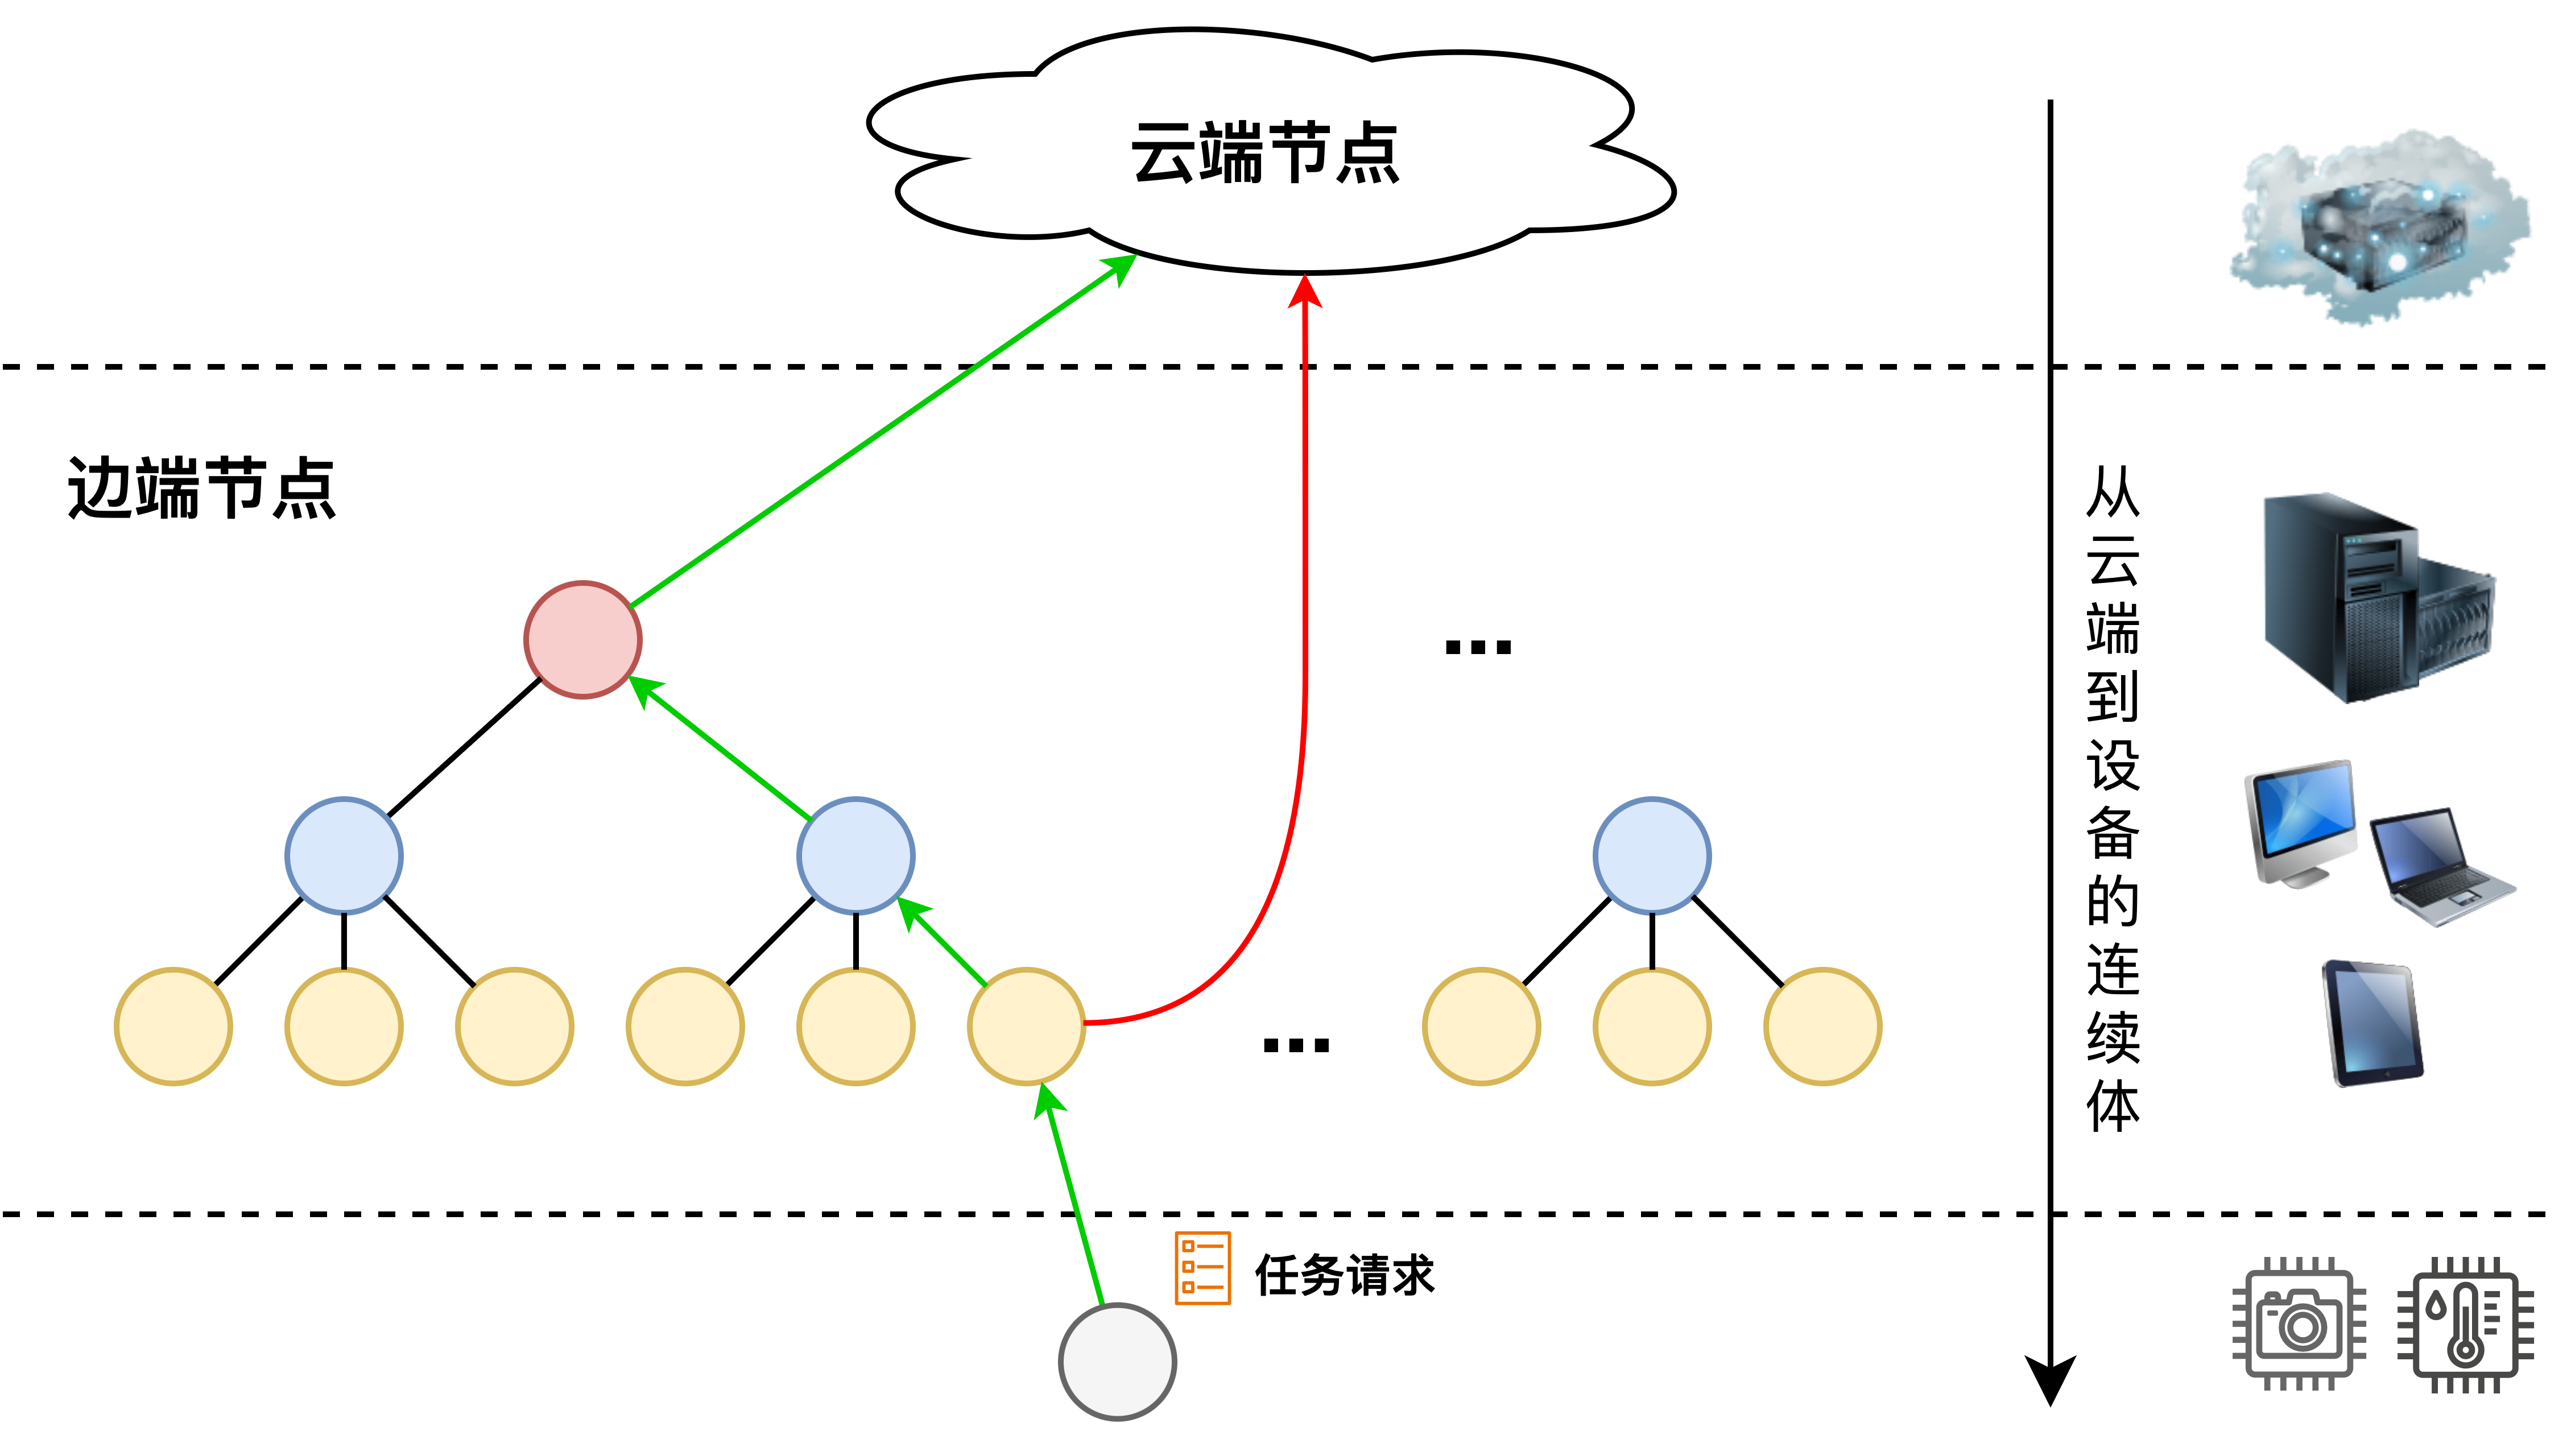
\includegraphics[width=0.8\linewidth]{pics/3-5schedule.png}
  \caption{云边协同AI推理分层调度示意图}
  \label{fig:3-5schedule}
\end{figure}

图\ref{fig:3-5schedule}展示了这种层次化的结构,其中所有边缘节点与云端之间形成了一个树状关系。当终端设备发起任务请求时,该请求会首先被发送至与其直接相连的边缘节点。如果当前节点有能力处理此任务,则直接执行并返回结果;若无法完成任务,则会将请求转发至上一级节点。这一过程由各层级的调度器协调完成,并优先考虑在本节点管理的子节点内寻找解决方案。此外,每个边缘节点还具备一定的灵活性,可以根据实际情况选择直接将任务请求发送至云端。这种方式虽然增加了直接通信的开销,但在某些特殊场景下,如子节点资源不足或延迟要求极高时,直接与云端协同可能更具优势。

\subsection{设备直连节点本地调度}

\begin{figure}[h]
  \centering
  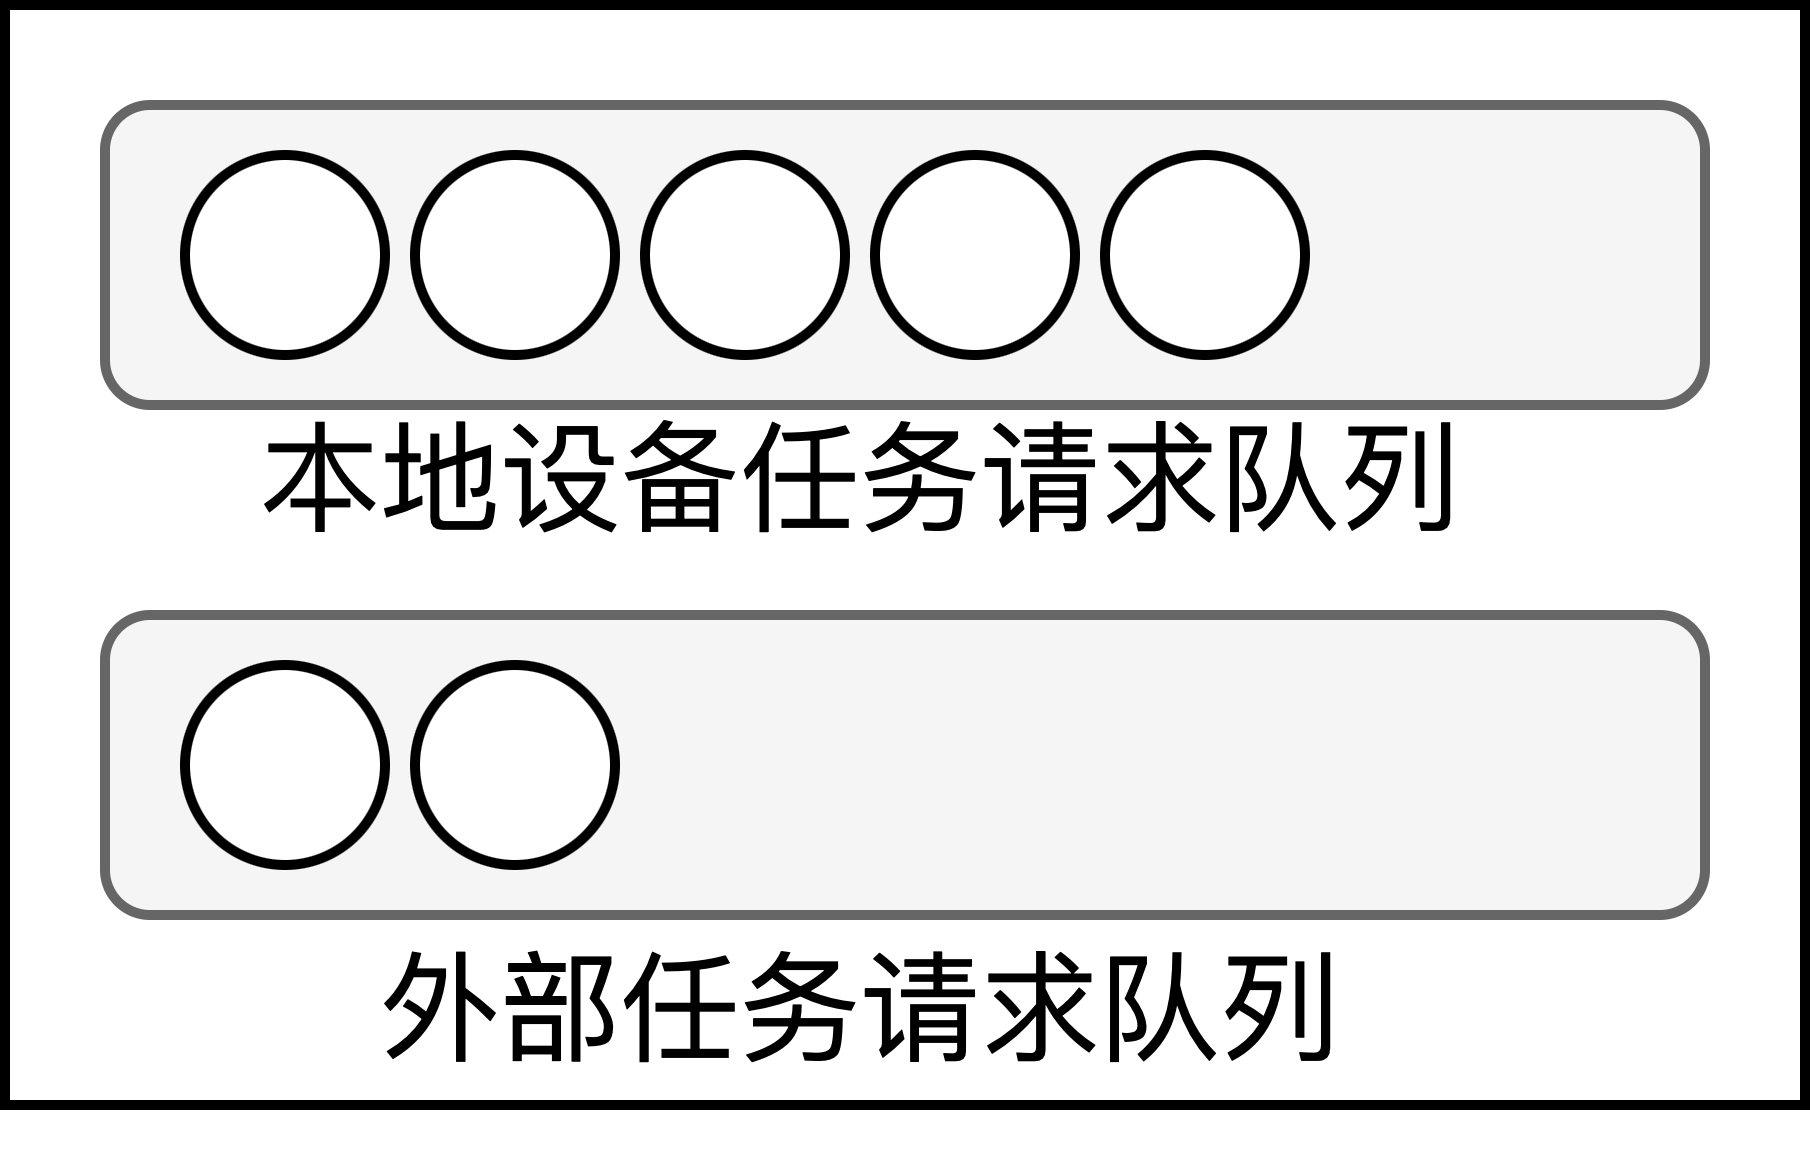
\includegraphics[width=0.4\linewidth]{pics/3-10本地调度.png}
  \caption{设备直连节点本地调度任务队列}
  \label{fig:3-10local}
\end{figure}

对于设备直连节点,本地存在两个任务队列:一个是本地设备的任务队列,另一个是上级节点分配的任务队列,如图\ref{fig:3-10local}所示。本地节点的调度器优先调度本地设备的任务请求,然后调度上级节点分配的任务请求。为了最小化外部流量,调度器首先处理单次采集量$\varsigma_\beta$ 最大的任务。

本文提出基于贪心策略的本地调度算法。该算法通过构建优先级队列,以本地设备单次数据采集量$\varsigma_{i\beta}$为依据,确保本地设备的数据流能够优先获得调度资源,同时有效减少跨节点传输的开销。在此基础上,算法还引入了弹性容量分配机制,在严格满足计算队列容量约束的前提下,动态调整数据分流比例。这一机制不仅能够保障本地服务质量,还能最大化系统吞吐量,从而在资源利用与性能需求之间实现平衡。具体算法流程如算法\ref{alg:local_scheduling}所示。

\begin{algorithm}[ht]
\caption{本地调度算法}
\label{alg:local_scheduling}
\begin{algorithmic}[1]
\REQUIRE  
  直连设备集合$\mathcal{D}_j$,  节点$v_j$在$t_\omega$时间窗的计算容量$C^{t_\omega}_j$, 设备流式数据特征元组$\{(g_i^{t_\omega}, \varsigma_{i\beta})\}_{d_i \in \mathcal{D}_j}$
\ENSURE  
  设备到节点的分流比例集合$\{z_{ij}^{t_\omega}\}$

\STATE 初始化分流比例 $z_{ij}^{t_\omega} \leftarrow 0,\ \forall d_i \in \mathcal{D}_j$  
\STATE 剩余可用容量 $R \leftarrow C_j^{t_\omega}$  

\STATE 生成设备优先级队列 $\mathcal{P} \leftarrow \textsc{Sort}(\mathcal{D}_j, \varsigma_{i\beta} \downarrow)$  
  \COMMENT{按单次数据量$\varsigma_{i\beta}$降序排序}

\WHILE{$\mathcal{P} \neq \emptyset$ \AND $R > 0$}
  \STATE 取出队首设备 $d_i \leftarrow \mathcal{P}.\textsc{Dequeue}()$
  \STATE 计算资源需求 $u_i \leftarrow g_i^{t_\omega} \times \varsigma_{i\beta}$ 
  
  \IF{$u_i \leq R$}
    \STATE $z_{ij}^{t_\omega} \leftarrow 1.0$ \COMMENT{全量本地化处理}
    \STATE $R \leftarrow R - u_i$ \COMMENT{更新剩余容量}
  \ELSE
    \STATE $z_{ij}^{t_\omega} \leftarrow R / u_i$ \COMMENT{按比例分配剩余容量}
    \STATE $R \leftarrow 0$ \COMMENT{触发资源耗尽状态}
  \ENDIF
\ENDWHILE
\RETURN $\{z_{ij}^{t_\omega}\}_{d_i \in \mathcal{D}_j}$
\end{algorithmic}
\end{algorithm}

算法\ref{alg:local_scheduling}的总体时间复杂度为$O(|\mathcal{D}_j| \log |\mathcal{D}_j|)$,其中通过排序函数 $\textsc{Sort}$ 构建设备优先级队列 $\mathcal{P}$的时间复杂度为 $O(|\mathcal{D}_j| \log |\mathcal{D}_j|)$,主循环逐一处理优先级队列中的设备的时间复杂度为 $O(|\mathcal{D}_j|)$。

\subsection{中间层次与云端全局调度}

\begin{figure}[h]
  \centering
  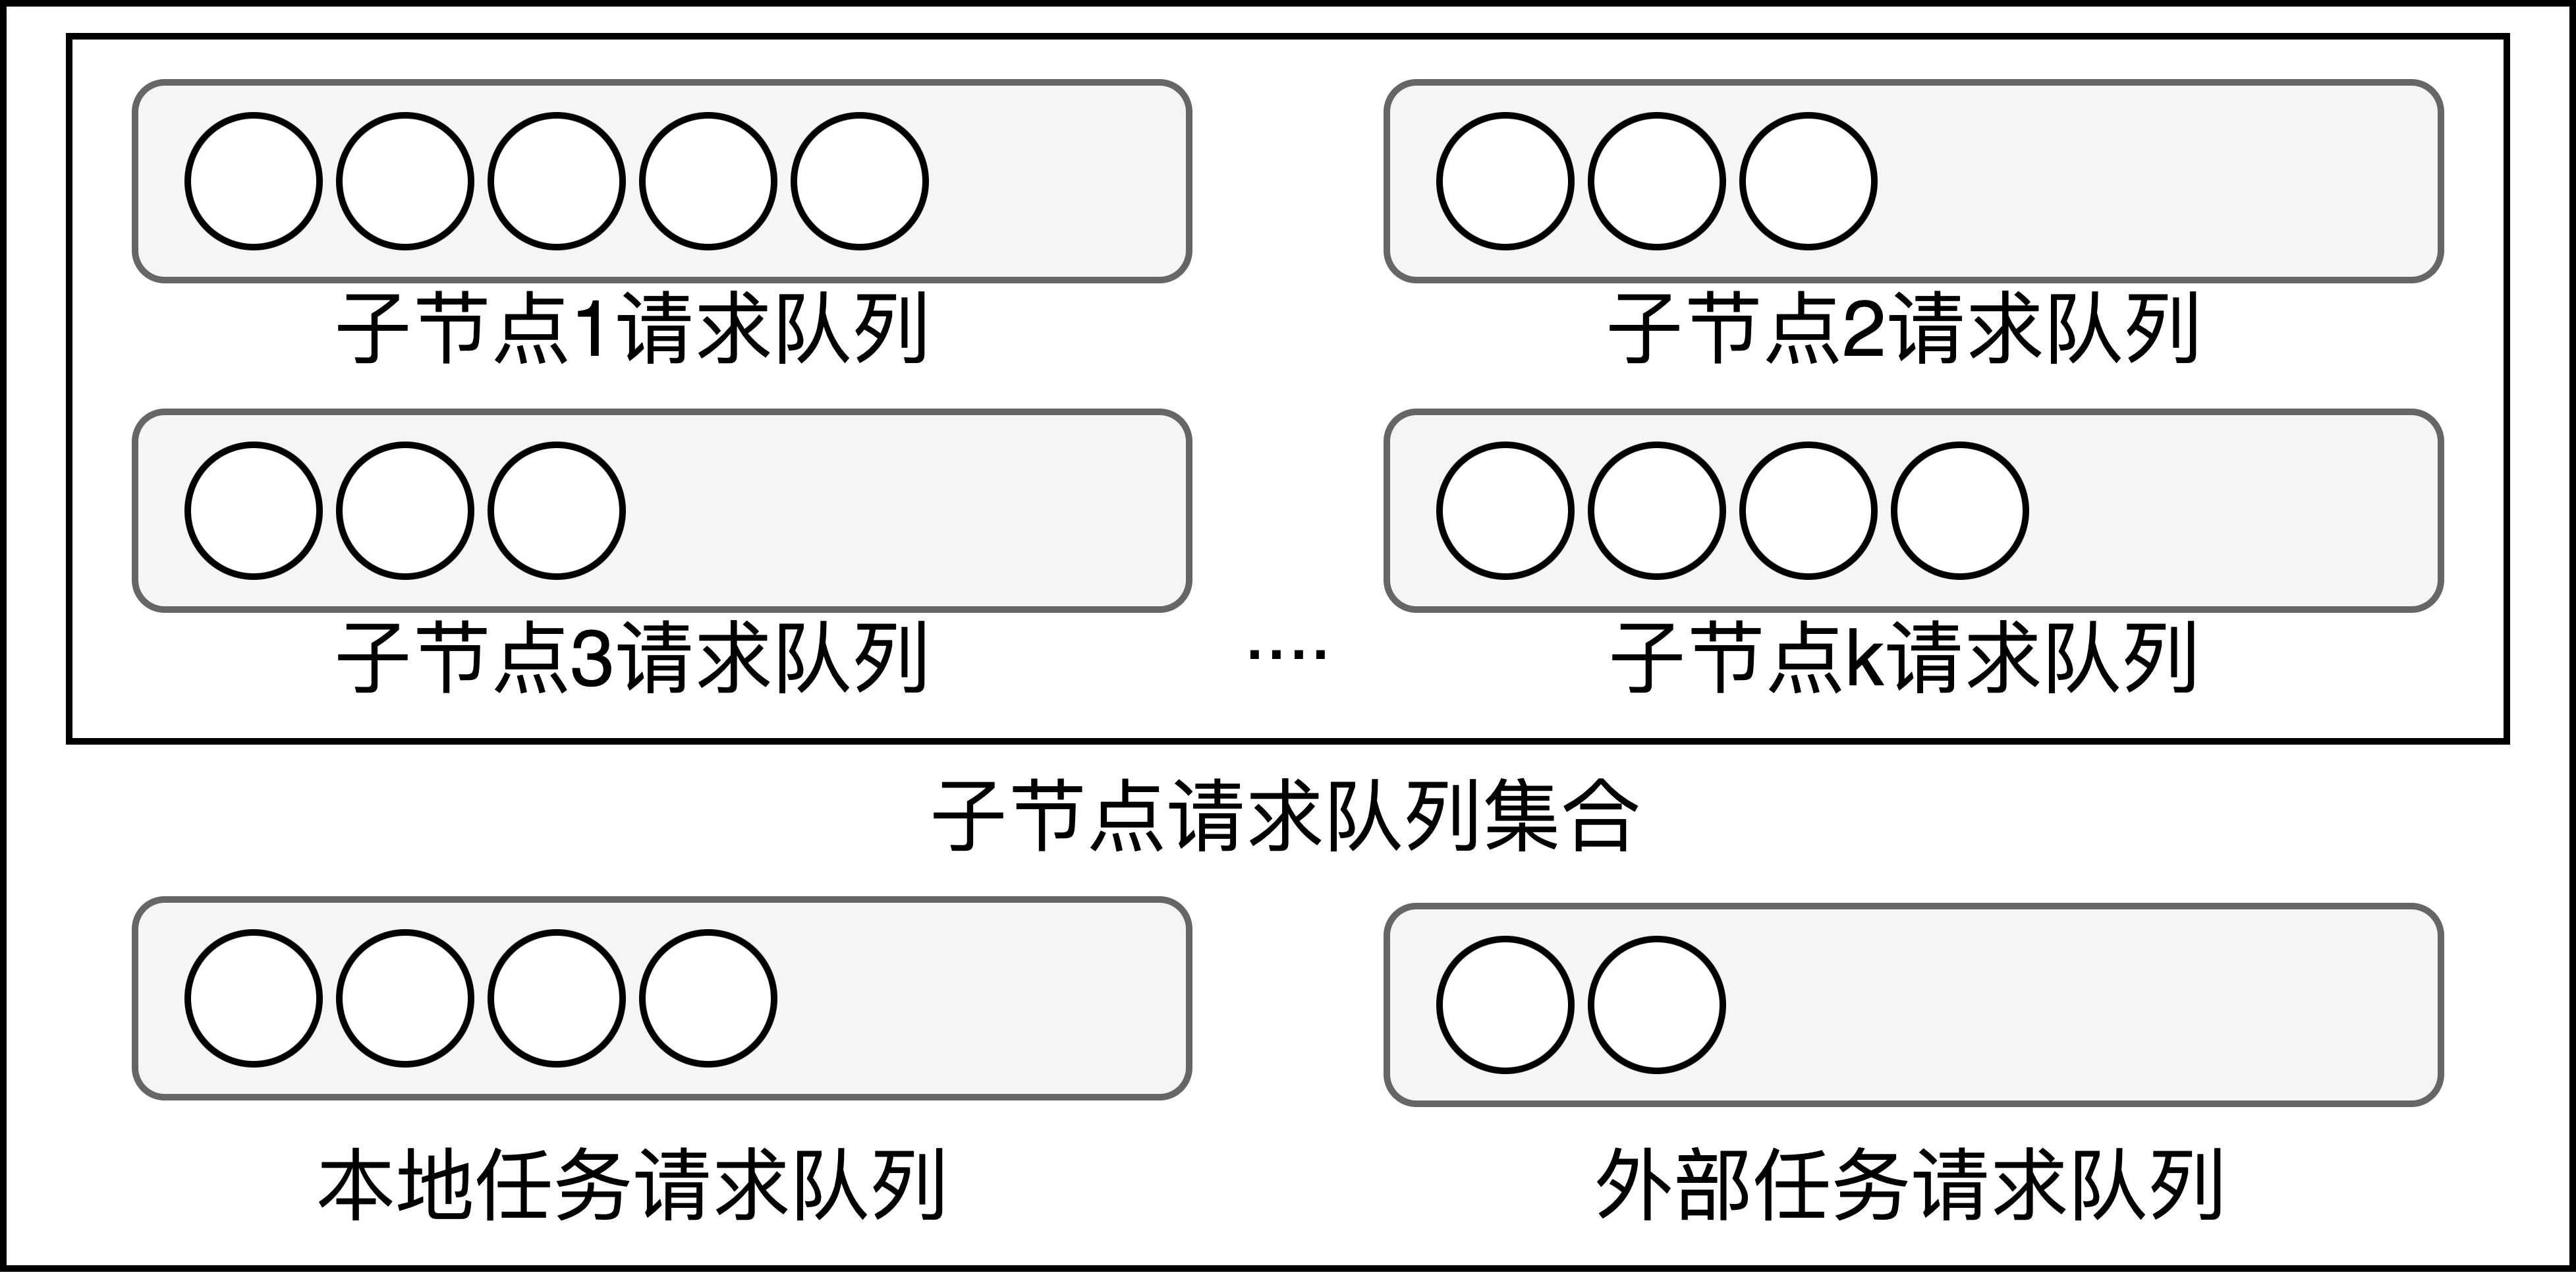
\includegraphics[width=0.8\linewidth]{pics/3-11集群调度.png}
  \caption{上层节点调度任务队列}
  \label{fig:3-11cluster}
\end{figure}

在每一级中间层次的节点中,都会维护其所有子节点的任务队列信息,同时记录自身的任务队列以及外部节点的任务队列信息。当某个设备的任务请求在下一级节点未能成功调度时,该请求会在当前层次的节点进行调度处理,如图\ref{fig:3-11cluster}所示。这种机制确保了任务能够在合适的节点层级得到及时响应,从而提高了系统的整体调度效率。为了最小化外部流量,中间层次调度器首先处理单次采集量$\varsigma_\beta$ 最大的任务。而云端为了实现最大化设备处理,可以优先处理最小的碎片任务,从而保证尽可能多的设备请求数据被完整处理。

本文提出了一种结合贪心策略与多维度优先级队列的中间层次与上层调度算法。该算法首先根据设备单次数据采集量或剩余数据量对流式数据进行优先级排序,构建初始优先级队列,在此基础上,针对每条流式数据,算法筛选出集群中具有剩余计算队列容量的候选节点,并进一步依据端到端时延建立时延优先队列。通过引入时延敏感度感知机制,算法有效降低了集群内部调度的总时延,同时满足任务的时延约束要求。此外,算法采用动态分配策略,在候选节点间按剩余容量比例分配数据流,既避免了单一节点过载问题,又最大化了集群内部计算资源的利用率。通过这一机制,算法在保证服务质量的同时实现了高效的资源调度与任务分配,具体流程详见算法\ref{alg:cluster_scheduling}。

\begin{breakablealgorithm}
\caption{中间层次与云端全局调度算法}
\label{alg:cluster_scheduling}
\begin{algorithmic}[1]
\REQUIRE  
  待调度数据流集合$\mathcal{F}_k$, 剩余容量$\{C^{t_\omega}_m\}_{e_{km} \in \mathcal{E}_k}$, 带宽参数$\{\Theta_{\text{total}}(e_{km})\}$, 单次采集量$\varsigma_\beta$
\ENSURE  
  数据流到集群节点的分流比例集合$\{z_{ikm}^{t_\omega}\}$

\STATE 初始化分流比例 $z_{ikm}^{t_\omega} \leftarrow 0,\ \forall f_i \in \mathcal{F}_k, e_{km} \in \mathcal{E}_k$  

\IF{中间层次调度}
\STATE 生成数据流队列 $\mathcal{Q} \leftarrow \textsc{Sort}(\mathcal{F}_k, \varsigma_\beta \downarrow)$  
  \COMMENT{按单次数据量$\varsigma_{i\beta}$降序排序}
\ELSIF{云端全局调度}
\STATE 生成数据流队列 $\mathcal{Q} \leftarrow \textsc{Sort}(\mathcal{F}_g, g_{i,\text{res}}^{t_\omega} \uparrow)$ 
    \COMMENT{按剩余数据量升序排列}
\ENDIF

\FOR{每个数据流 $f_i \in \mathcal{Q}$} 
  \STATE 获取候选节点集 $\mathcal{N}_i \leftarrow \textsc{FilterNodes}()$  
    \COMMENT{筛选兼容且有剩余容量的节点}
  \STATE 生成时延优先级队列 $\mathcal{M}_i \leftarrow \textsc{Sort}(\mathcal{N}_i, \Theta_{\text{total}} \uparrow)$  
    \COMMENT{按端到端时延升序排序}
  \STATE 剩余待分配量 $r_i \leftarrow g_{i,\text{res}}^{t_\omega}$

  \WHILE{$r_i > 0$ \AND $\mathcal{M}_i \neq \emptyset$}
    \STATE 取出队首节点 $e_{km} \leftarrow \mathcal{M}_i.\textsc{Dequeue}()$
    \STATE 可用容量 $a_m \leftarrow C^{t_\omega}_m - \sum_{f_j \in \mathcal{F}_k} z_{jkm}^{t_\omega} \cdot g_{j,\text{res}}^{t_\omega}$
    
    \IF{$a_m \geq r_i$}
      \STATE $z_{ikm}^{t_\omega} \leftarrow r_i / g_{i,\text{res}}^{t_\omega}$  
        \COMMENT{全量分配给当前节点}
      \STATE 更新节点容量占用 $C^{t_\omega}_m \leftarrow C^{t_\omega}_m - r_i$
      \STATE $r_i \leftarrow 0$
    \ELSE
      \STATE $z_{ikm}^{t_\omega} \leftarrow a_m / g_{i,\text{res}}^{t_\omega}$  
        \COMMENT{按剩余容量比例分配}
      \STATE 更新节点容量占用 $C^{t_\omega}_m \leftarrow 0$
      \STATE $r_i \leftarrow r_i - a_m$
    \ENDIF
  \ENDWHILE
\ENDFOR
\RETURN $\{z_{ikm}^{t_\omega}\}$
\end{algorithmic}
\end{breakablealgorithm}

算法\ref{alg:cluster_scheduling}的总体时间复杂度为$O(|\mathcal{F}_k| \log |\mathcal{F}_k| + |\mathcal{F}_k| \cdot |\mathcal{E}_k| \log |\mathcal{E}_k|)$,其中生成数据流优先级队列的时间复杂度为$O(|\mathcal{F}_k| \log |\mathcal{F}_k|)$,而针对每个数据流的候选节点筛选和时延排序的时间复杂度为$O(|\mathcal{E}_k| \log |\mathcal{E}_k|)$。主循环部分的时间复杂度为$O(|\mathcal{F}_k| \cdot |\mathcal{E}_k|)$,确保了算法在大规模集群环境下的可扩展性。

\section{本章小结}

本章系统研究了云边协同环境下的AI推理调度优化问题。首先构建了云边协同AI推理调度模型,形式化定义了终端设备、计算节点、AI负载实例等核心组件,阐述了数据流驱动的动态调度机制,为分层调度策略的设计奠定了理论基础。接着提出了云边协同 AI 推理分层调度的思想,然后介绍了设备直连节点本地调度和中间层次与云端全局调度的机制,形成了完整的资源协调流程。最后针对各层级特点,设计了差异化优化方法:本地调度采用基于优先级排序的弹性容量分配算法,动态调整分流比例以最大化资源利用率;中间层次节点通过多维度优先级队列融合时延敏感度感知机制,降低集群内调度时延并减少跨域流量;云端全局调度有效降低资源碎片化并提升系统吞吐量。
